\chapter{Introduction}
%
% This is the introduction~\cite{deb01, pyprop}\ldots



\pagebreak
\section{Introduction}

``We won’t have a society if we destroy the environment''

Margaret Mead

The commencement of industrial revolutions in the last centuries is closely related to the outbreak of environmental damages and harmful manipulation of ecosystems. Environmental issues are actual and can lead to serious consequences for human beings and ecosystems. Lack of knowledge and uncertainty make these issues to be easily hidden behind other short-term industrial and political concerns for decision making authorities. 
 
The contribution of human $\mbox{CO}_2$ emissions as green-house gas in the climate change has been shown by studies such as \cite{houghton2001climate}. The underground sequestration of the $\mbox{CO}_2$ produced from the localized sources like power-plants and oil and gas recovery sites is proposed as a possible solution to reduce the rate of $\mbox{CO}_2$ emission into the atmosphere \cite{hitchon1999sedimentary,bradshaw2001geological}. The required technology for this solution is close to what is in use in the oil and gas and mining industry, which is technically feasible. However, there are some challenges that are specific to the carbon storage operations. The time and space scales in these problems are larger. The risk of leakage of stored $\mbox{CO}_2$ up to the surface via conductive features like fractures and faults and the manmade features such as leakage through the ill-plugged wells and broken cap-rock due to high pressure imposed to the system during the injection operations is a major concern. 

The main objectives of carbon storage operations are to maximize the storage size in a shorter injection operations and to minimize the risk of leakage of the stored $\mbox{CO}_2$. The $\mbox{CO}_2$ storage must be studied from different aspects. The relevant tasks are divided between government and private section, research organizations and industry. It is the task of research community to investigate the safety of $\mbox{CO}_2$ sequestration and provide the methodology for $\mbox{CO}_2$ fate prediction \cite{bachu2000sequestration}.

Bachu discusses the road map of site selection for geological $\mbox{CO}_2$ sequestration \cite{bachu2000sequestration}. He defines the process in four steps: to assess the general suitability of the site, to perform the inventory study on the source point and storage location and the operational transport issues, and finally to investigate the safety and assess the capacity of the storage. Issues about safety and storage capacity are looked at differently from the perspective of immediate and ultimate results and local and global locations. For example, when talking about the risk of leakage, we might consider the leakage through ill-plugged wells or fractures during the injection time as the immediate risk. On the other hand, the leakage which is made by plume migration long time after the injection and contamination to the other aquifer systems are considered as ultimated risks. 

In order to predict the $\mbox{CO}_2$ injection fate, it is crucial to study the dynamics of flow in the medium. By quantifying the acting forces, one can predict the flow attributes under different circumstances. It seems convenient to replace the geological heterogeneous medium with an equivalent homogeneous medium. However, proper modeling of geological heterogeneity is a major control on reservoir assessment and carbon storage studies \cite{eaton2006importance,bashore1993importance,melick2009incorporating,milliken2008effect}.

The work in this thesis is tackling the fundamental uncertainty in geological description used in modeling of $\mbox{CO}_2$ storage problems. The work is reported in a series of papers, and the objective is to perform a sensitivity analysis on variational geological parameters used to describe the geology of shallow-marine depositional systems. Although the focus is on the shallow-marine depositional systems, but the procedure can be implemented for any other systems of interest. 

We start the introduction section by discussing the global warming and its causes, and the carbon storage as an interim proposed solution to mitigate the increasing level of industrial $\mbox{CO}_2$ emission to the atmosphere. That follows by discussing the work-flow of the works reported in the thesis. A brief overview of the literature is given and the position of the work is discussed. 

Geological description and geological uncertainty are the main part of the work and a report is given in these regards. Uncertainty definitions and typology can be controversial from various perspectives. We review a systematic definition for uncertainty from the literature and after that, the geological uncertainty and parameters are described.

The introduction to the thesis continues by a report on flow simulation assumptions taken in the work and information about the modeling of multiphase flow in the problem. We use a comprehensive set of flow responses that monitor the performance of the operation and requirements to achieve the objectives of a typical carbon storage problem, with a special emphasis on the injection and early migration of $\mbox{CO}_2$ in the medium.  

In order to be able to analyze the variations in the output of the system and quantify the global sensitivity of responses to the uncertain input, we use a response surface method to simulate the flow responses. This proxy model is then used in a Monte-Carlo process. The introduction section ends by introducing the Matlab functions used in the calculation work-flow. 

\section{Carbon storage}

There are a number of theories that explain the causes of climate change. Milankovich theory relates the energy received from the sun to the  cyclical variation of earth orbit around the sun, and earth rotation around its axis \cite{foukal2006variations}. The earth orbit changes eccentricity between circular and elliptical. This influences the difference between earth and sun, and on it's maximum influence can lead to about $20\%$ difference in the energy received from the sun. The second variation occurs in the rotation of earth around its plane axis. This rotation wobbles approximately every $13600~\mbox{years}$ and the summer solstice switches from June to January. Also, a tilt variation of earth rotational axis happens approximately after every $41000~\mbox{years}$. This can cause warmer winters and colder summers in the high latitudes \cite{foukal2006variations}. 

% Volcanic eruptions mostly have a temporary effect on the climate. Based on the available observation records, the sulfur dioxide produced from the volcanic activity stays in the atmosphere about three years after eruption and reacts with the water vapor to make a layer blocking the transmission of sun radiations towards earth. This in general results in a cooling effect which lasts as long as the dense haze vapor layer exists there.

The solar radiation changes by small amount of $0.1\%$~over a $11$ year cycle. Also on the scales of tens to thousands of years the variations in the earth orbit results in seasonal changes and that in the old past caused glacial and inter-glacial cycles.

The theory of green house effect relates the earth climatic change to the fact that the long wave radiation from earth back to atmosphere is absorbed by the green house gases, mainly carbon dioxide, water vapor, and methane existing in the atmosphere. This results in trapping of heat energy and an increase in atmosphere temperature level (Figure~\ref{fig:grHsGs}) \cite{foukal2006variations}.

\begin{figure}
  \centering
  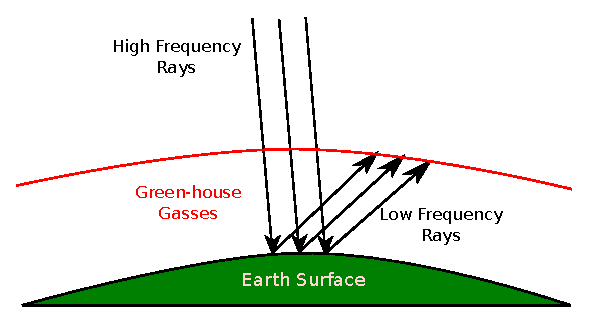
\includegraphics[width=0.65 \linewidth]{./figurer/G-H_gasses} 
  %
  \caption{Green-house gases work like a blanket trapping the heat received from the sun.}
  \label{fig:grHsGs}
%
\end{figure}

Human manipulations in the nature has led to about $100~\mbox{ppm}$ increase in carbon dioxide level in the atmosphere. Most scientists believe that we are already experiencing the global warming due to green house effects. The IPCC Second Assessment report states that the climate change in the late $19^{th}$ century is most likely due to anthropogenic causes. 

Carbon capture and storage (CCS) has got a major attention in the industry and the scientific communities. Based on International Energy Agency (IEA) the cost of mitigating climate change by $2050$ is estimated to be $70\%$ higher without implementing CCS.

The CCS is considered as an interim solution, because it is valid due to fossil fuel consumption, and the long term strategy of replacing fossil fuel with renewable energy will terminate the validity CCS. Therefor, stressing the CCS has to be done in a reasonable fashion such that it does not slow down the research for renewable energy. Another concern regarding the CCS is the acceleration of coal and fossil fuel consumption with the excuse of availability of CCS technology.

\begin{figure}
  \centering
  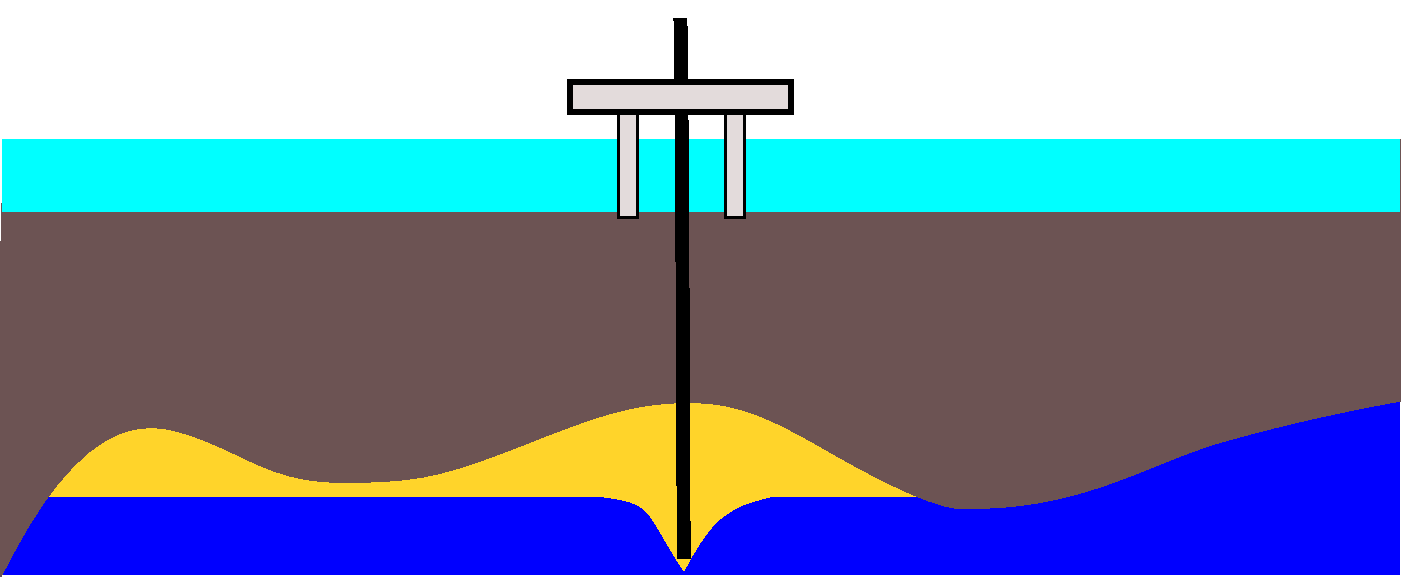
\includegraphics[width=0.65 \linewidth]{./figurer/platform} 
  \caption{Geological sequestration is a proposed solution for mitigating the industrial $\mbox{CO}_2$ emissions.}
  \label{fig:platform}
%
\end{figure}


Sequestration of CO$_2$ in the roof of oceans and also in the deep underground aquifers are the available options for permanent storage of $\mbox{CO}_2$. Large availability of storage places and potential for almost permanent storage makes the geological sequestration as a practical option (Figure \ref{fig:platform}). Nevertheless, this alternative is not free from economical, social and industrial concerns.  

In the last decades, the scientific communities have been putting efforts into convincing the social perceptions about feasibility of these operations. A fair public acceptance must be based on social awareness. Any plan to increase the acceptance level in a society starts by measuring the current knowledge level of that society. 

The EU has conducted a survey to assess the public awareness in $12$ European states. This survey is published in the recent Eurobarometer report in May $2011$. People's awareness and acceptance of climate change and its causes, and the methods to avoid or mitigate the problems, in particular the CCS technology, was examined in the survey. Majority of European participants are either fairly or very well informed about causes and consequences of climate change. However, the awareness of CCS in between the European respondents was low. Two third of participants in the survey have not heard at all about the CCS. 

The same survey suggests that the overall trust in Europe in the sources of information regarding the CCS is best in universities and scientific research communities. Governments are investing in research, not only to move toward industrialization of CCS, but also to make it well received by public. This highlight the importance of researching the storage of $\mbox{CO}_2$ and the way it is needed both for industrial demands and social inquiries.
\subsection{Geological storage}
% DIFFERENT FLOW REGYMES
% two phase flow
% relative permeability
% dimensional analysis



\section{Modeling procedure}

Predicting the fate of $\mbox{CO}_2$ storage requires an intensive amount of work within a comprehensive procedure to identify and quantify the relevant uncertainty and assess the risks and consequences resulting from the uncertainty propagation through the system. The procedure starts with geological description and continues with modeling of flow in geological formations. After constructing a deterministic flow modeler, the stochastic nature of the problem is analyzed by studying the variation in the model outcome due to uncertainties in the system. 

\begin{figure}
  \centering
  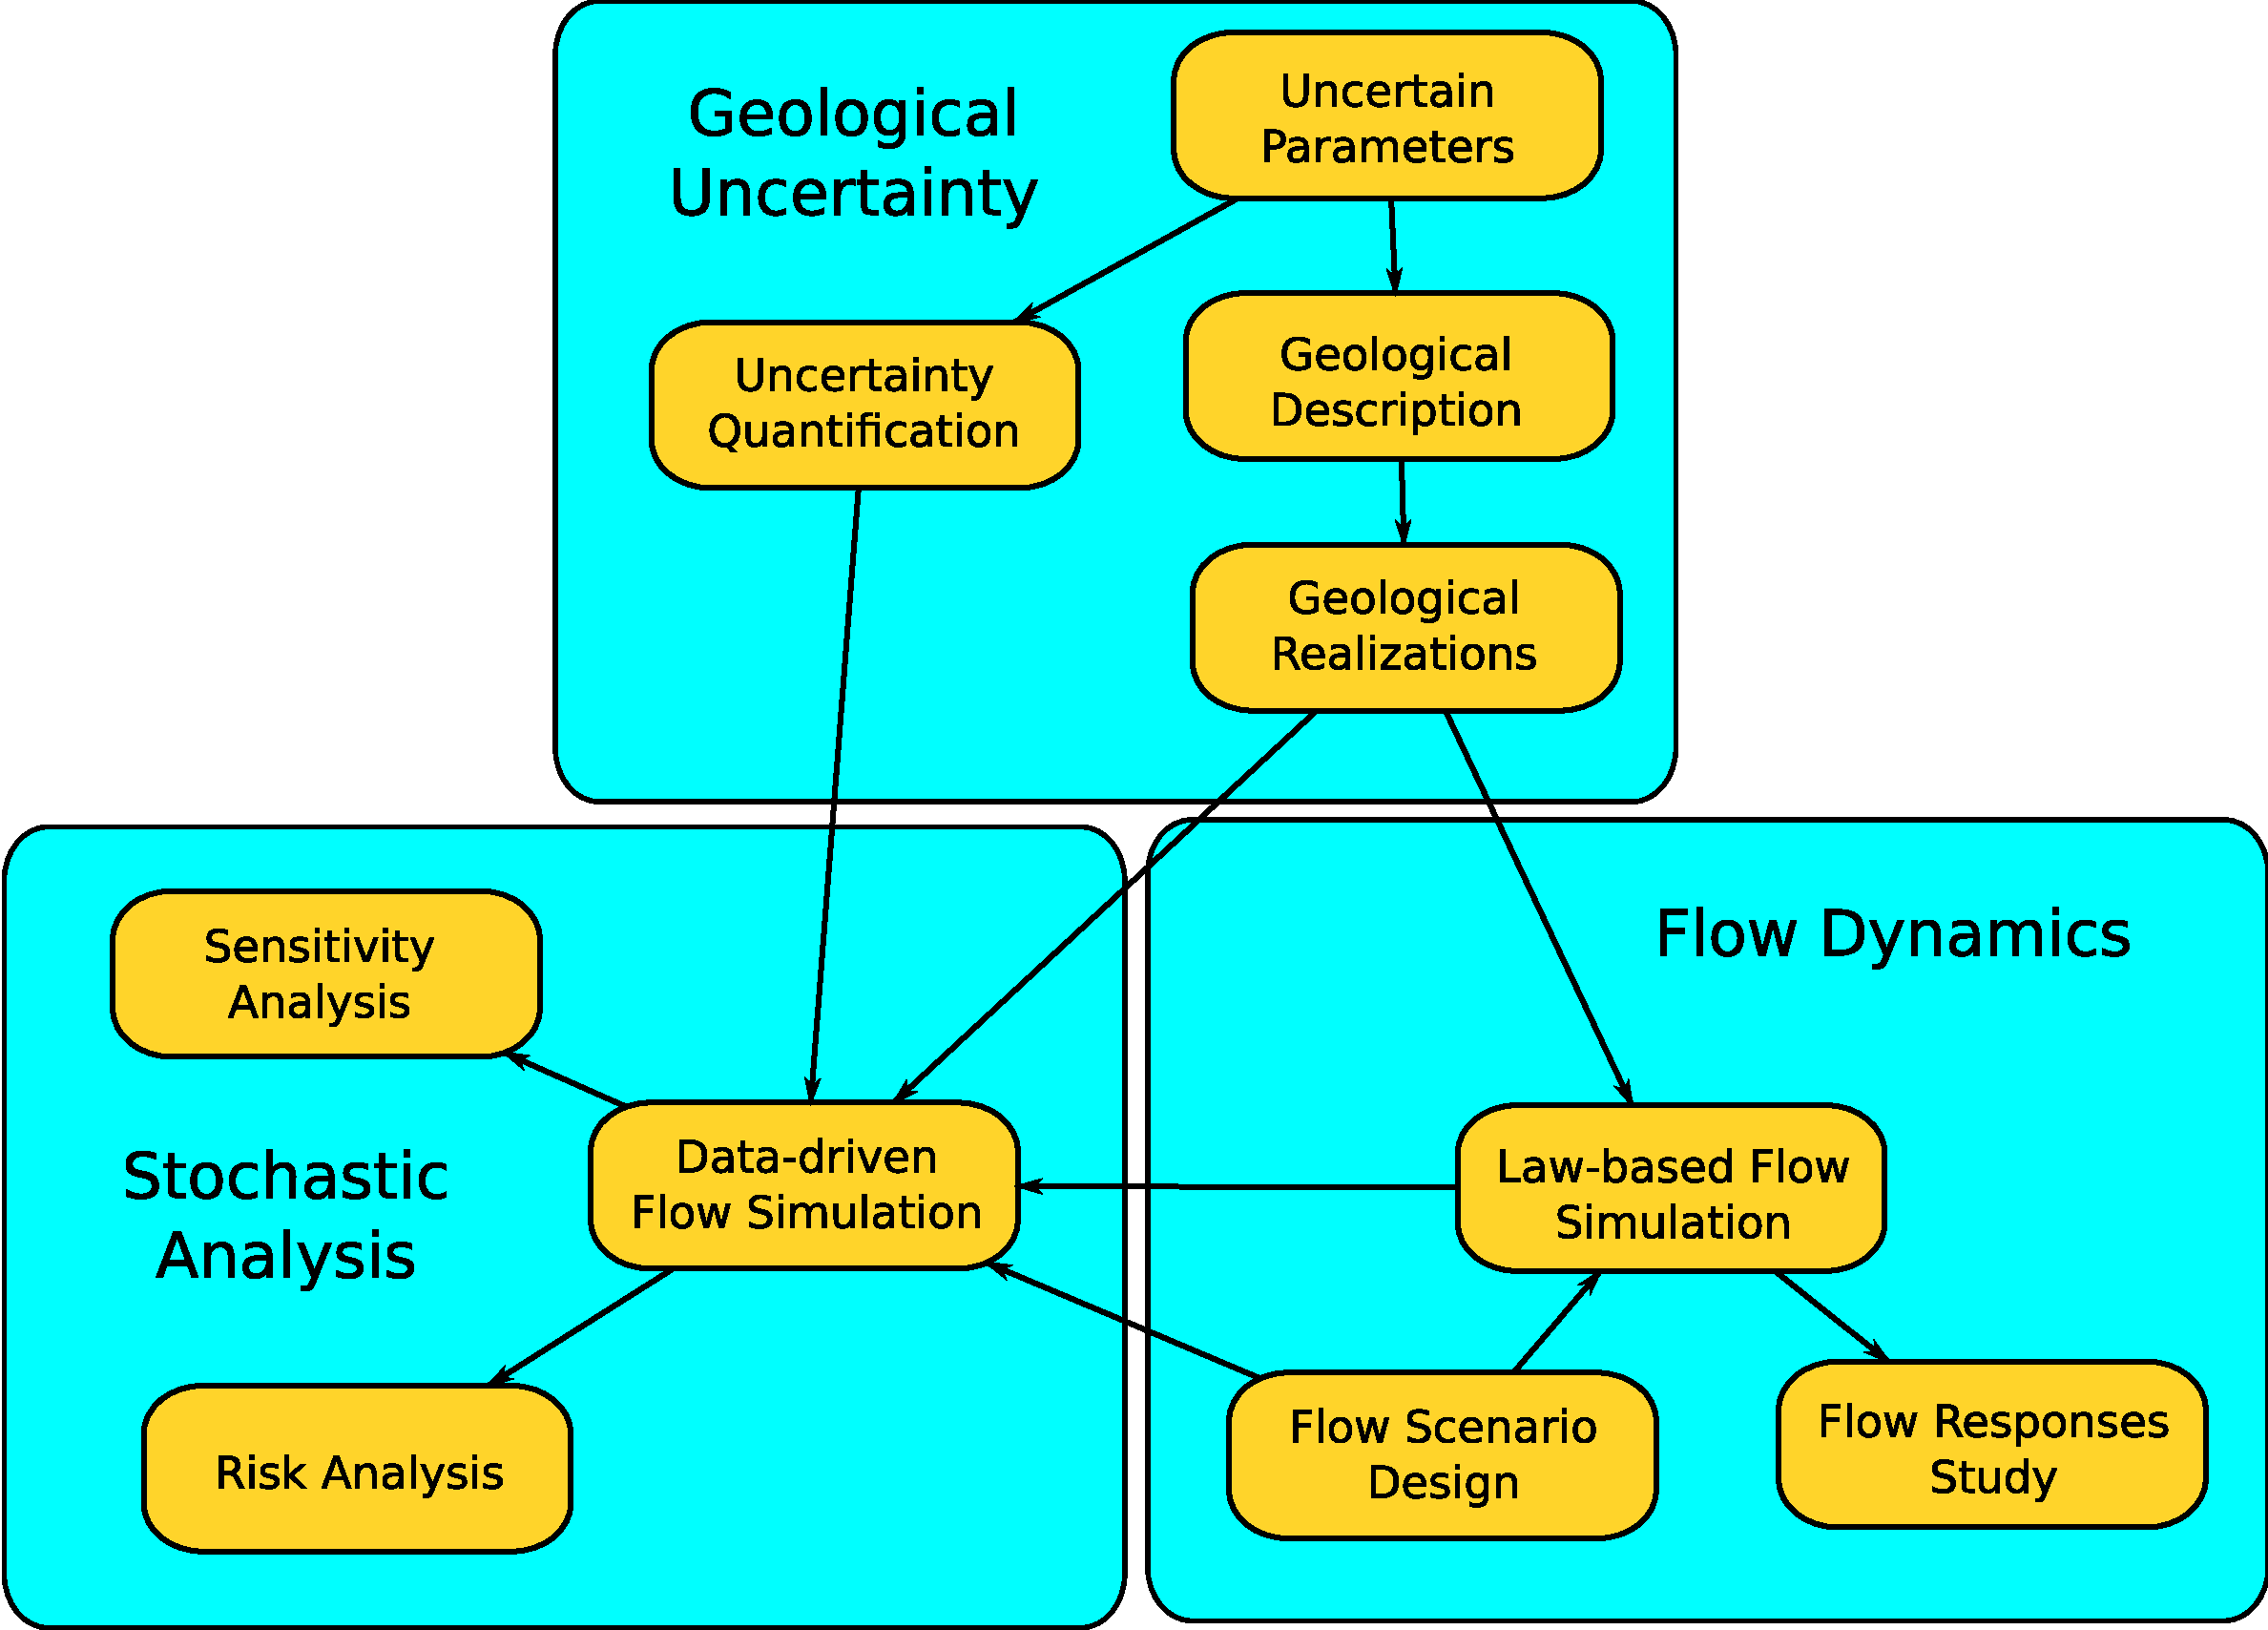
\includegraphics[width=0.95 \linewidth]{./figurer/prc2} 
  
  %
  \caption{Modeling procedure diagram.}
  \label{fig:prc}
%
\end{figure}

Figure \ref{fig:prc} shows the work-flow of modeling the uncertainty consequences that is implemented in the work of this thesis. The steps are categorized in three parts: geological uncertainty, flow dynamics, and stochastic analysis. The relations between steps are plotted by arrows in the flow-chart. In this section, we briefly describe each step and more details will follow in the next sections.

\textbf{Uncertain parameters:} In the first step, we identify the uncertain parameters of the model that we are interested to study their influence in the modeling outcome. In general, we might have a rough understanding about the significance of parameters influence and choose them based on this knowledge in order to quantify this significance. Also, it is possible that our knowledge of model sensitivity to the parameters is limited. Then, in a conservative approach we choose larger number of parameters and by doing a primary sensitivity analysis with a fast technique, we filter out the important parameters. Herein, the focus is on the geological parameters.

\textbf{Uncertainty quantification:} After identification of the uncertain geological parameters, we assign a likelihood to each of the parameters. Although it might be possible to find a universal likelihood for a geological parameter, but most of the uncertainties in geology depend on the location of the study. The uncertainty enters the modeling in the form of parameter frequency histograms. The conventional practices consider an analytical distribution function to be assigned to the parameters. However, the sampling procedure normally ends in a scarce frequency histograms that are difficult to justify their representation with an analytical distribution function.

\textbf{Geological description:} Geological uncertainty study is normally done by series of runs to measure the sensitivity of the model to the parameter variations. The variations in one geological parameter must be modeled in a realistic fashion, such that it represents an actual geological feature. Geological description is very essential in modeling the uncertainty. Results are valid, only if the geology used in the work-flow is representative of reality. The process of geological description results in a large number of realizations to be used in the next steps of the study.

\textbf{Flow scenario design:} Flow dynamics depends on the definition of flow problem in the model. Initial and boundary conditions must be defined and an injection scenarios must be specified. The injection scenarios are implemented within all the selected geological realizations in the study. Possible simplifying physical assumptions will be taken here.

\textbf{Law-based flow modeling:} After defining the injection problem, we simulate the flow dynamics in the chosen realizations. The flow behavior is demonstrated in a set of unknown attributes that can be found by solving the flow equations which are based on physical laws: mass, momentum, and energy conservations. The simplifying physical assumptions define the formulation of equations. Numerical techniques are used to solve the flow equations.

\textbf{Data-driven flow modeling:} Modeling the flow dynamics via formulations of physical laws normally results in complicated equations with large degrees of freedom. The computational cost of solving these equations is high, in particular if these models are used for uncertainty related studies that require a large number of simulations to cover the variation in the uncertain parameters. 

The alternatives for such studies are methods that are mathematical expressions describing dependency of the unknown flow attributes to the uncertain parameters. The so called data-driven methods, are mathematical functions that are specified by correlating a set of known flow attributes to their corresponding uncertain parameter values. The tuning process can be performed by running a set of selected simulations by the costly law-based methods and tuning the data-driven function by the those run results. Because these methods are designed to be only and directly dependent on the uncertain parameters, they are normally low in computational costs. However, they may exhibit the pitfall of not following the physical rules in some cases with unrealistic run results. 


\textbf{Flow responses study:} Once the simulation results are obtained from the flow modeling procedure, it is possible to calculate the important flow responses from simulation results. The fate of carbon storage and assessment of the operations can be inferred from these responses. Storage volume capacity and rate, and leakage risk are evaluated from flow responses.

\textbf{Sensitivity analysis:} To enhance the efficiency of the work-flow, sensitivity analysis is used to rank the most influential parts of the modeling. Simplifying assumptions can be taken for non-influential parameters and parts in the modeling. A global sensitivity analysis that covers the entire uncertainty intervals for the input parameters is used to demonstrate the significance of parameter influence in the system behavior.

\textbf{Risk analysis:} The propagation of input parameters uncertainty can be investigated by analyzing the results of simulations run on the input parameters with considerations for probabilities. With fast data-driven flow simulators, it is possible to perform a comprehensive Monte-Carlo process via a large number of simulations  over input uncertainties.

\section{Geological description}


The central part of a successful $\mbox{CO}_2$ storage fate modeling is to provide plenary aquifer models that depict the geological heterogeneity in a realistic manner. This requires having an inclusive understanding about model sensitivity with respect to different geological parameters and quantifications of geological uncertainty and its impacts on the process. 

The conventional practice of geological modeling includes using geostatistical models inferred from the scarce available rock property distributions to populate the entire medium with those rock attributes. Through a sensitivity analysis work-flow, the geostatistical modeling might be performed to generate large number of realizations that depict the heterogeneity variations that are to be examined for flow behavior. First step of geostatistical modeling is yo go from more to less information to model the variations within space in the main directions of the model, a considerable amount of information related to heterogeneities may not be conserved and get reproduced in the next property population steps. It is possible that two different heterogeneity patterns produce the same geostatistical model. The geostatistical model does not represent a unique reservoir image and if we do not include additive information in the process, the heterogeneity texture will not be represented accurately resulting in a different local and global flow behavior in the model than what happens in a real aquifer. 

Most of the works done on heterogeneity effects in $\mbox{CO}_2$ storage studies are either related to a case study with a deterministic geological structure or using geostatistical equiprobable cases in which the heterogeneity is simulated by using the conventional variograms \cite{nicot2008evaluation,LGH1992611,le2010corrective,LGH1993959,rutqvist2002cap,rutqvist2007}. However, a more realistic uncertainty analysis requires variational aquifer images that themselves are realistic. In other words, the heterogeneity expressed in lithological textures must be embedded in the image of variational modeling parameters, such as permeabiliy or porosity. The primary  attention in our work has been on this issue and to provide a more realistic way of geological uncertainty analysis for $\mbox{CO}_2$ sequestration by including information of geological features and textures in the process. 

\subsection{Uncertainty}

Quantifying geological uncertainty is a dominant step in the underground flow studies. However, the topic can be controversial in the applied terminology from different perspectives. In this section, we start by a brief introduction to uncertainty to give a systematic review based on \cite{walker2003defining}. The section continues by a discussion dedicated to geological uncertainty.

Walker et al. define uncertainty as being 'any deviation from the unavailable ideal of completely deterministic knowledge of the relevant system'. But measuring this deviation can be controversial with reference to different perspectives. Thus, it is not a surprise to find two articles within uncertainty assessment context that show inconsistency in the uncertainty terminology, classifications, or measurements. Regulations and policies providing decisions on concert matters need to be based on framework, work-flow, and basis for knowledge. With these motivations, Walker et al. proposed conceptual basis for uncertainty management. Within model-based uncertainty context, alternative policies are examined for their outcome. Identifying outcomes of interest, aligned with policy goals, requires determining a structure for the system and the work-flow in the model. 

% Uncertainty can be distinguished in three dimensions: location, level, and nature. Sources of uncertainty manifest themselves within the structural framework of the system and the logic of model formulation. Location of uncertainty can be classified in a number of categories. The context can be uncertain in identification of system boundaries. Defining the model and the dependency rules can include levels of uncertainty. For example, some influential physical phenomena may be neglected within the modeling process.  A typical uncertainty is the uncetainty that is embedded in the model inputs. Another location in the process that sources of uncertainty can exist is the parameters defined in the model. Parameters are constants in the model that may be universal parameters, a priori chosen parameters, or calibrated constants of the model. Finally, uncertainties can exist in the model outcomes.

% \begin{figure}
%   \centering
%   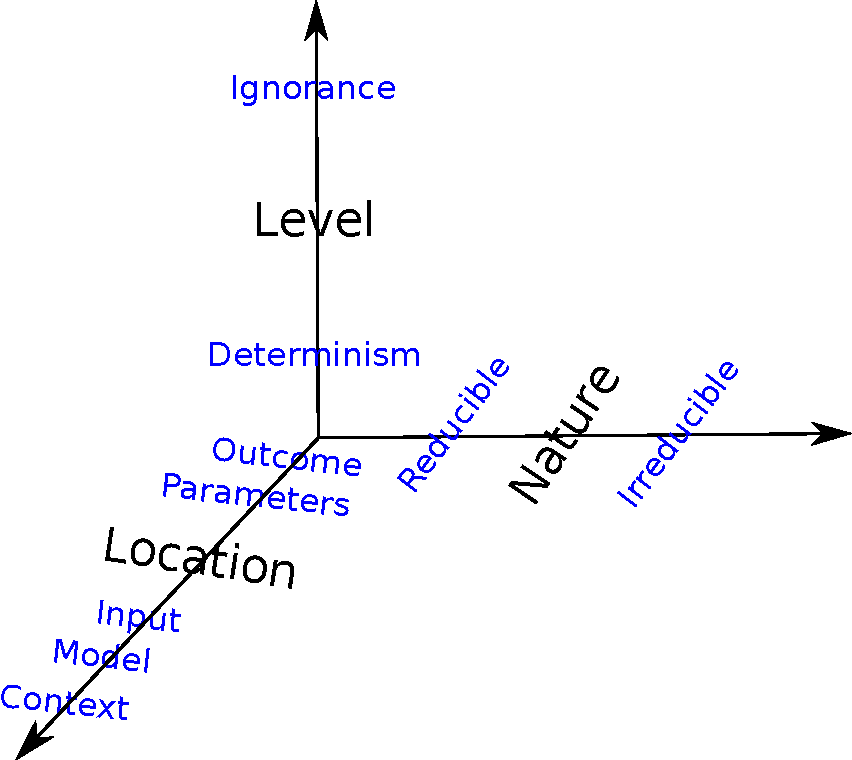
\includegraphics[width=0.65 \linewidth]{./figurer/uncertainty} 
%   %
%   \caption{Uncertainty dimensions based on the definitions by Walker \cite{walker2003defining}.}
%   \label{fig:uncertainty}
% %
% \end{figure}

% Uncertainties can change in level in a spectrum between two extremes: ideal determenistic knowledge and total ignorance. Level improvement goes from total ignorance, to the recoginsed ignorance, which is the fundamental uncertainty of mechanisms. When the knowledge of mechanisms and forcing drives development exist with uncertainty in the level of balance, we are not certain about scenarios that may lead to outcomes of interests. Next, we have the level at which uncertainty is reduced to statistical analysis, with certainty in knowing model formulation and mechanisms. Nature of uncertainty can be defined as if it is reducible or irreducible ( Figure ~\ref{fig:uncertainty}). 

In carbon storage context, policies and regulations are needed as preventive measure for undesired consequences. Politicians, industrial partners, and scientists contribute in a work-flow of decision making at which uncertainties about operational consequences have to be identified and treated systematically. Scientists have the role to identify uncertainties at different locations of the process, and to quantify the level of those uncertainties, and finally to reveal the nature of generated uncertainties in the system. The policy analysts and regulators develop alternative policies and within the work-flow of collaboration between different partners these policy alternatives are assessed to be ranked with respect to the desirable goals.

$\mbox{CO}_2$ injection operation comes with massive uncertainties. The most obvious, and at  the same time, important uncertainty is the lack of adequate geological knowledge. Transmissibility of rocks in the medium, structural traps and topography, and amount of pore volume in the medium are all information that must be derived from a geological description and are vital in modeling the underground flow performance. Geomechanical modeling of the layers and injectivity of wells determine the feasibility and safety of injection operations. Flow performance forecast depends on the fluid properties, rock-fluid interaction, and physical modeling of multiphase flow in the medium. Sources of uncertainty can exist in different places such as parameters, modeling formulation, or physical simplifying assumptions. Modeling procedure can be highly biased and subjective, leading to random variations and uncertainties in the outcomes.


\subsection{Geological parameters}

In the series of works reported here, the aim is to indicate the significance of appropriate geological descriptions in the injection and early migration of $\mbox{CO}_2$ in deep aquifers.  From the flow modeling perspective, sources of geological uncertainty can manifest themselves in the rock parameters that go in the flow equation such as permeability and porosity. This can easily lead to the inaccurate impression that to represent the geological uncertainty it is enough to directly randomize these parameters and study the variances in the flow solutions. This approach might work in simple geological models, but it can fail to give plausible results in the realistic heterogeneous problems. The geological uncertainty is rooted within structural and depositional description of geological formations and a comprehensive study on heterogeneity variability is needed.

In response to the EU priorities of reducing time to first oil and of improving overall hydrocarbon recovery efficiency, the interdisciplinary SAIGUP study was initiated to increase the understanding of the influence of geological uncertainties in oil field recoveries. SAIGUP stands for 'sensitivity analysis of the impact of geological uncertainties on production forecasting in clastic hydrocarbon reservoirs'. The context in the SAIGUP is defined for shallow-marine depositional systems. The main objective of the SAIGUP has been to perform a quantitative sensitivity analysis to measure the impact of sedimentological and structural variations withing geological descriptions on the oilfield recovery estimates \cite{howell2008sedimentological,manzocchi2008sensitivity,matthews2008assessing}. 

Sedimentological variability is modeled in small and large scales and combined to provide a range of impact in a realistic representation of reservoir heterogeneities. Structural aspects are modeled via fault modeling within geological description. Faults are considered in different levels of intensity, orientation, and transmissibility. Five waterflood scenarios are designed in various injection-production well patterns, resulting in simulated production behavior for over $35000$ full-field reservoir models. All models have the same total pore volume and vary in few number of grid geometries. 

Although these models are designed to study the impact of geological heterogeneity on oil recovery, it is feasible to implement carbon storage scenarios in them. Therefore, we have selected a number of parameters from the setup and varied these parameters by combining different levels. Five geological factors are considered for $\mbox{CO}_2$ storage studies. These features are lobosity, barriers, aggradation angle, progradation, and fault. In the following, we describe each feature briefly.


\textbf{\textit{Lobosity}}: Lobosity is defined by the plan-view shape of the shore-line. As a varying parameter, lobosity indicates the level at which the shallow-marine system is dominated by each of
the main depositional processes. Two depositional processes are considered in the SAIGUP study: fluvial and wave processes. The higher amount of sediment supply from rivers relative to the available accommodation space in the shallow sea, the more fluvial dominant the process will be. As the river enters the mouth of the sea, it can divide into different lobes and branches. Wave processes from the sea-side smear this effect and flatten the shoreline shape. Less wave effect produces more pronounced lobe shapes around the river mouths. 

Very high permeability and porosity can be found in the channeling branches, while dense rock with low permeability fills the space between them. Reservoir quality decreases with distance from the shore-face. We expect that the level of lobosity can have a considerable effect on the CO$_2$ injection and plume size in the aquifer. In this study, models of three levels of lobosity are used: flat shoreline, one lobe and two lobes, see Fig.~\ref{fig:lobCauses}.

 
\begin{figure}[tbp]%
  
  \subfloat[Lob1.]{\label{fig:lob1}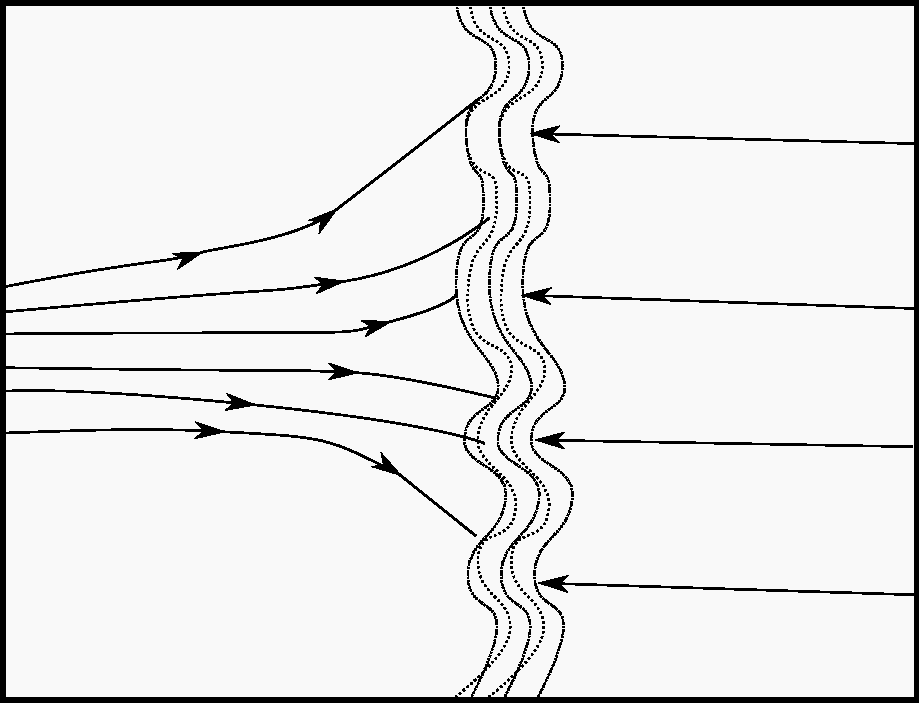
\includegraphics[width= 0.3 \linewidth]{./figurer/lob_1}} \hspace{0.5cm}
  \subfloat[Lob2.]{\label{fig:lob2}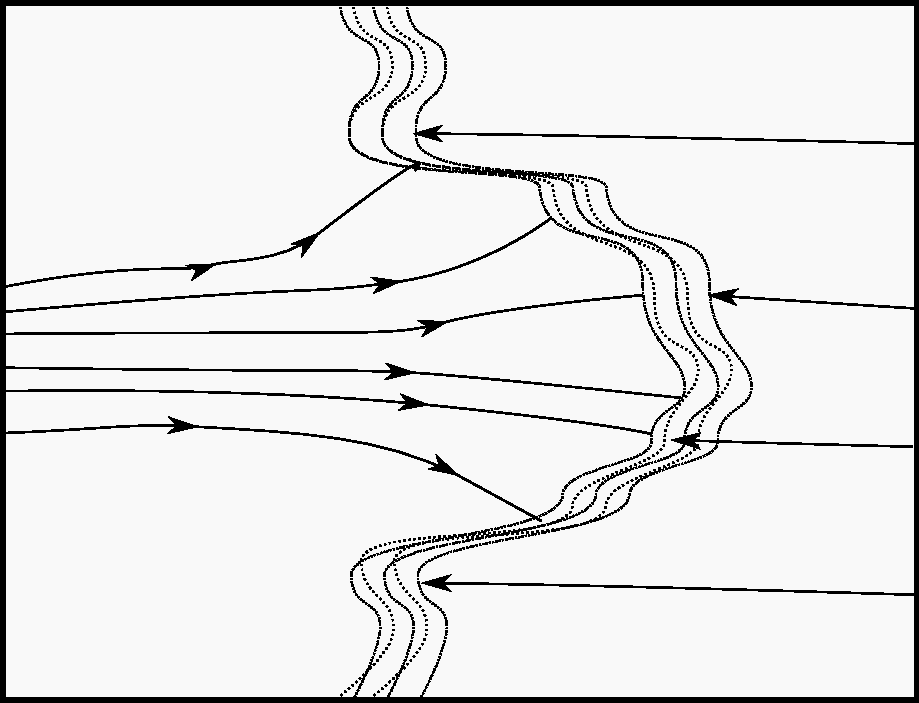
\includegraphics[width= 0.3 \linewidth]{./figurer/lob_2}}\hspace{0.5cm}
  \subfloat[Lob3.]{\label{fig:lob3}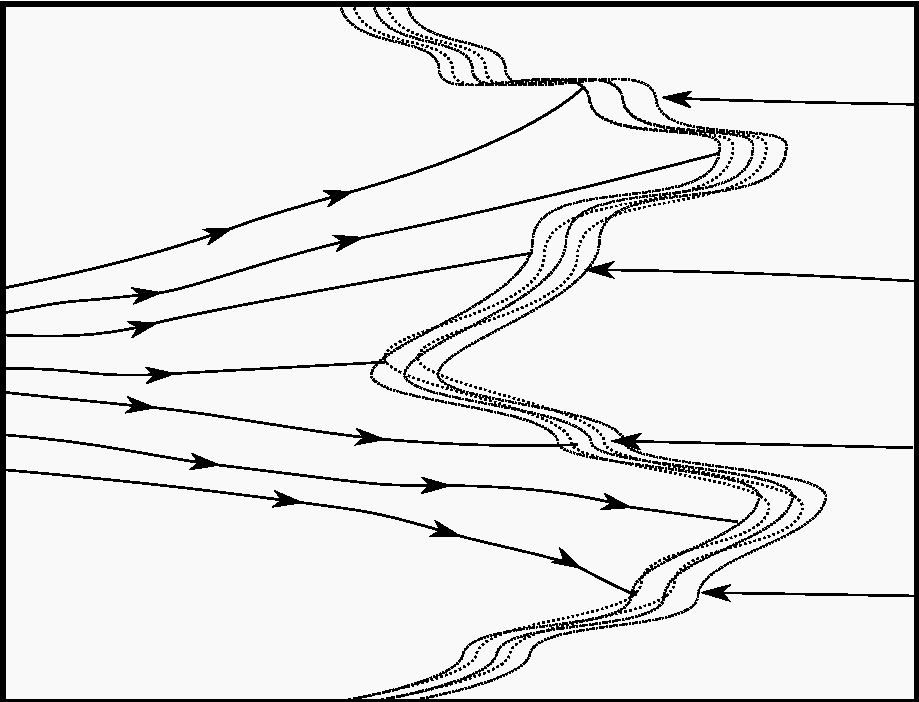
\includegraphics[width= 0.3 \linewidth]{./figurer/lob_3}}

  \caption{Lobosity levels are defined based on the shoreline shape, which is caused by the interplay between fluvial and wave forces.}
 \label{fig:lobCauses}
\end{figure}

\textbf{\textit{Barriers}}: 
Periodic floods result in a sheet of sandstone that dips, thins, and fines in a seaward
direction. In the lower front, thin sheets of sandstone are inter-bedded with the mudstones
deposited from suspension. These mud-draped surfaces are potential significant barriers to
both horizontal and vertical flow.  In the SAIGUP domain used here, these barriers were modeled by
transmissibility multipliers in three levels of zero value percentage: low (10\%), medium
(50\%), and high (90\%). We use the same variations in this study, see Fig.~\ref{fig:barriers}.


\begin{figure}[thb]
  \centering
  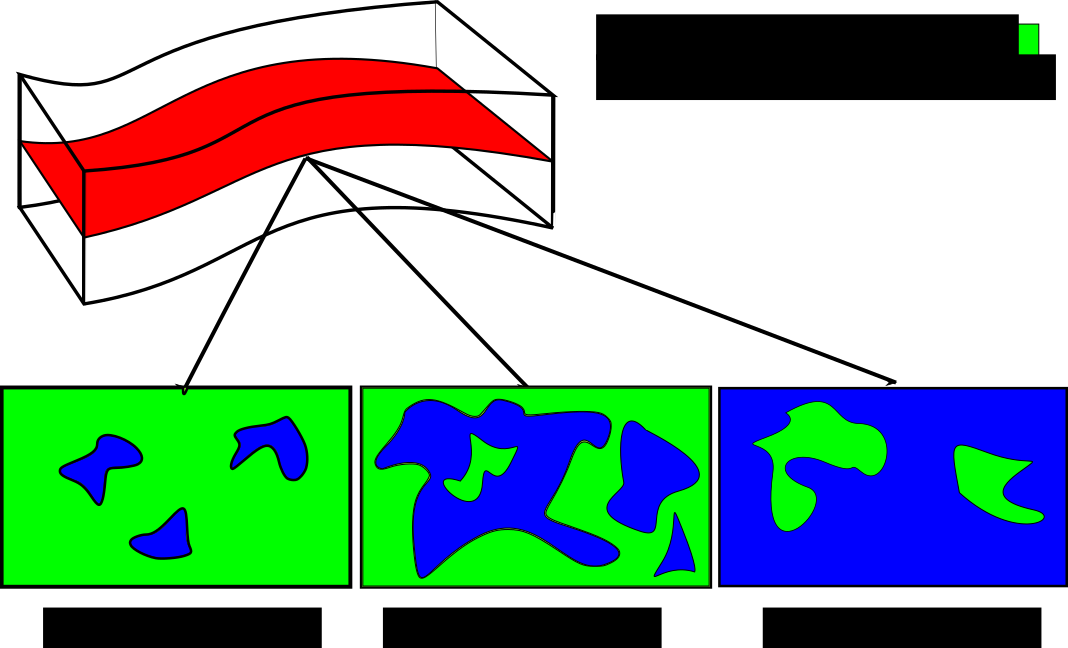
\includegraphics[width=0.65 \linewidth]{./figurer/barrier} 
  %
  \caption{Barrier levels caused by periodic floods.}
  \label{fig:barriers}
%
\end{figure}

\textbf{\textit{Aggradation angle}}: 
In shallow-marine systems, two main factors control the shape of transition zone
between the river and the basin: amount of deposition supplied by the river and the
accommodation space that the sea provides for these depositional masses. One can imagine a
constant situation in which the river is entering the sea and the flow slows down until
stagnation. The deposition happens in a spectrum from larger grains depositing earlier in
the land side to fine deposits in the deep basin. If the river flux or sea level
fluctuates, the equilibrium changes into a new bedding shape based on the balance of these
factors.

\begin{figure}[thb]
  \centering
  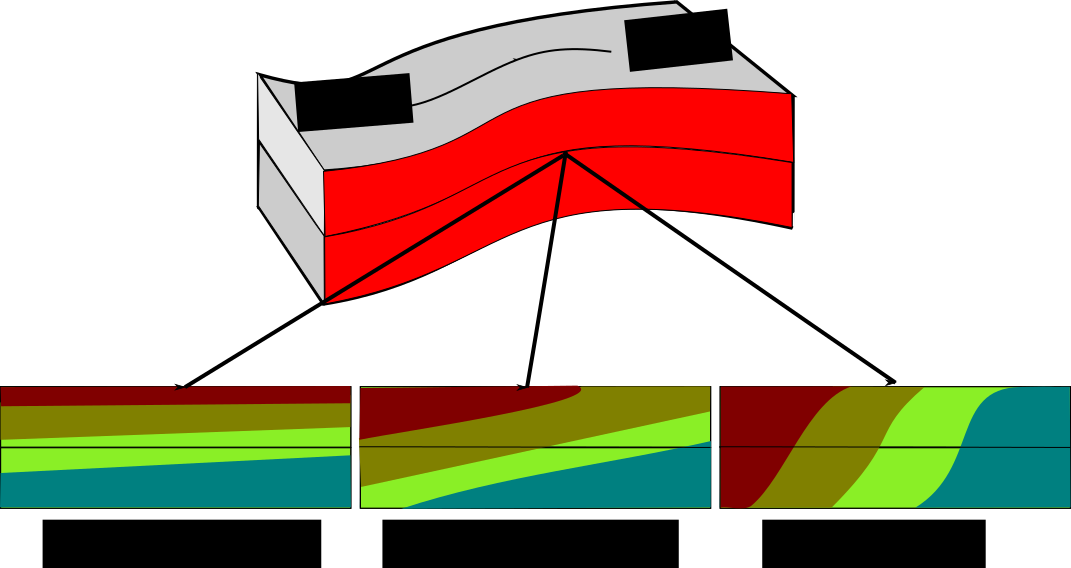
\includegraphics[width=0.65 \linewidth]{./figurer/agr} 
  %
  \caption{Aggradation angle levels.}
  \label{fig:agrLvl}
%
\end{figure}

In the SAIGUP study, the progradational cases are considered in which, for example, the
river flux increases and shifts the whole depositional system into the sea. The angle at
which the transitional deposits are stacked on each-other because of this shifting, is
called aggradation angle. Three levels of aggradation are modeled here: low, medium and
high (Fig.~\ref{fig:agrLvl}). As we will observe later, aggradation can have a dramatic
influence on the injection and migration process.

\textbf{\textit{Progradation}}: 
The final factor varied is the progradation or the depositional-dip
direction. Two types are considered here: up and down the dominant structural dip. Since
the model is tilted a little, this corresponds to the lobe direction from flank to the
crest or vice-versa (Fig.~\ref{fig:proLvl}). This has a potential influence on the CO$_2$ flow
from the injection point up to the crest.


\begin{figure}[thb]
  \centering
  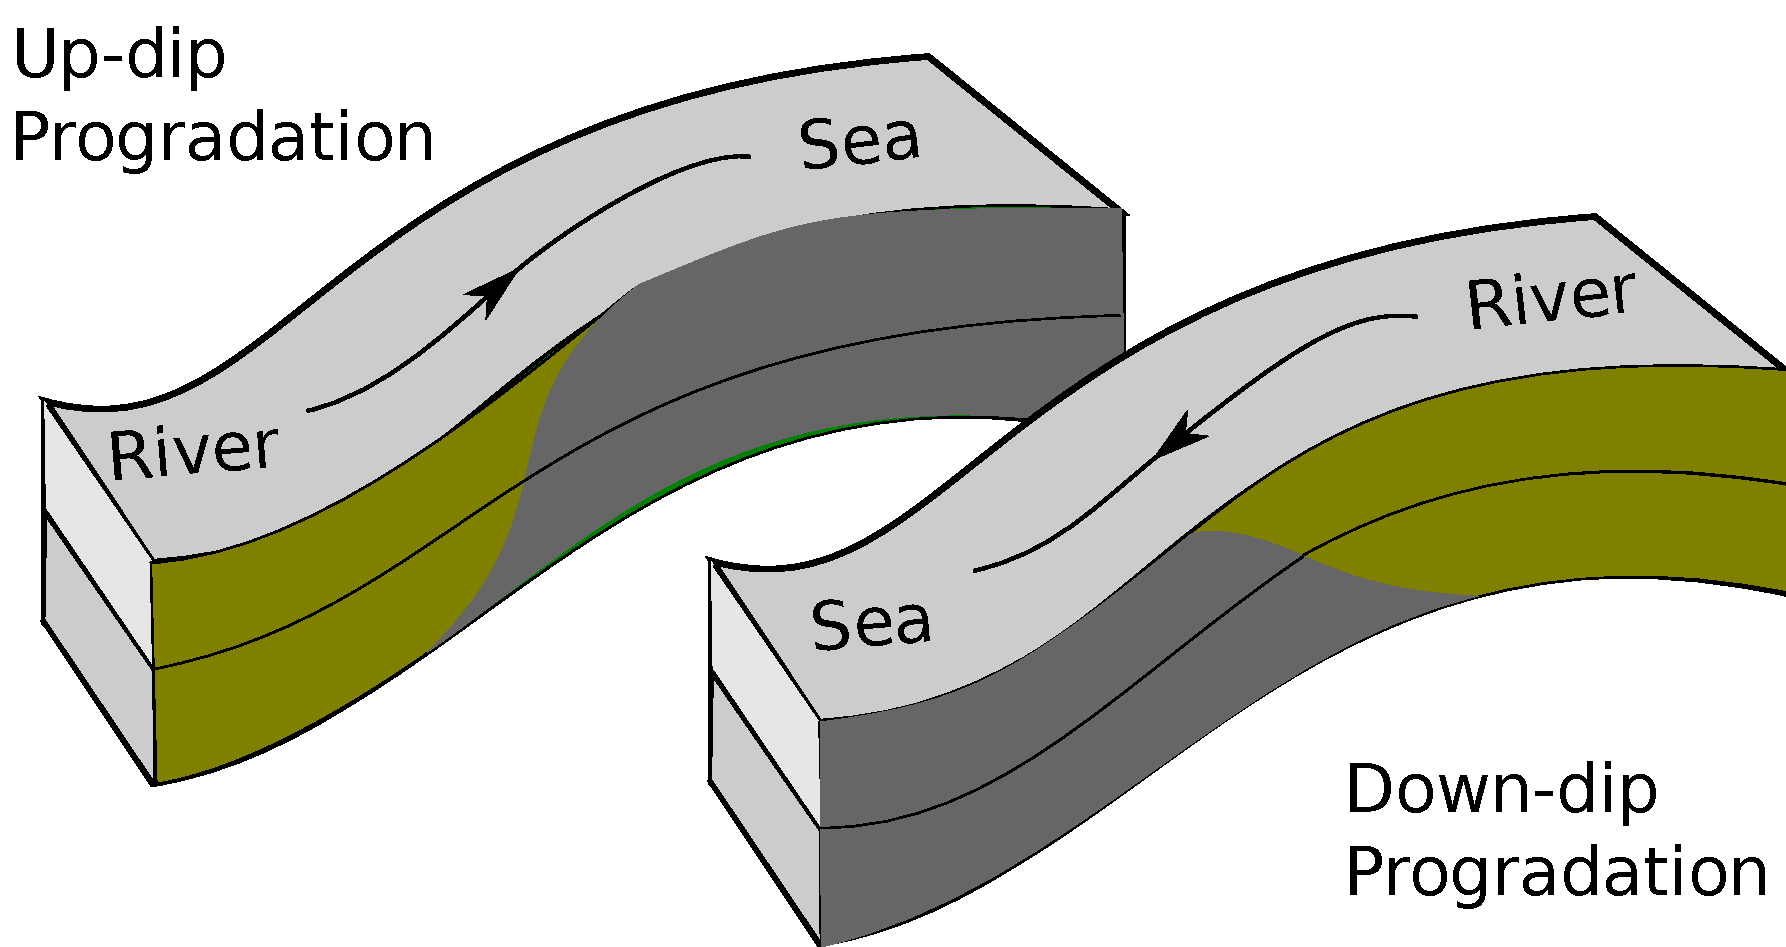
\includegraphics[width=0.65 \linewidth]{./figurer/progradation} 
  %
  \caption{Progradation levels.}
  \label{fig:proLvl}
%
\end{figure}

\textbf{\textit{External pressure support}}:

Defining the boundary condition of the aquifer of interest can influence the flow behavior in the system. One advantage of aquifers for carbon storage is the availability of large aquifers to provide the required accommodation space. Computational costs make that more feasible to model the flow locally and in the part of the aquifer that is going through more pronounced changes in flow behavior. Therefor, we can choose the boundaries of the model inside the aquifer in a volume that is containing the injection wells and the areas effected by them. Hydrostatic open boundary condition is a choice for the system boundaries to include the aquifer parts that fall outside the boundaries (Fig. \ref{fig:bkw}).

The underground network of aquifer systems can be connected via geological channeling and conductive features. Some aquifers might be active and connected to the surface and expand in volume by variations in water influx due to  seasonal rains. This can impose an external force on the system boundaries considered in a storage problem. Fig. \ref{fig:bkw} shows the water influx through the boundaries of the system due to external aquifer activities. We consider the external support by imposing a higher pressure than the hydrostatic pressure on the boundary of the model.

\begin{figure}[thb]
  \centering
  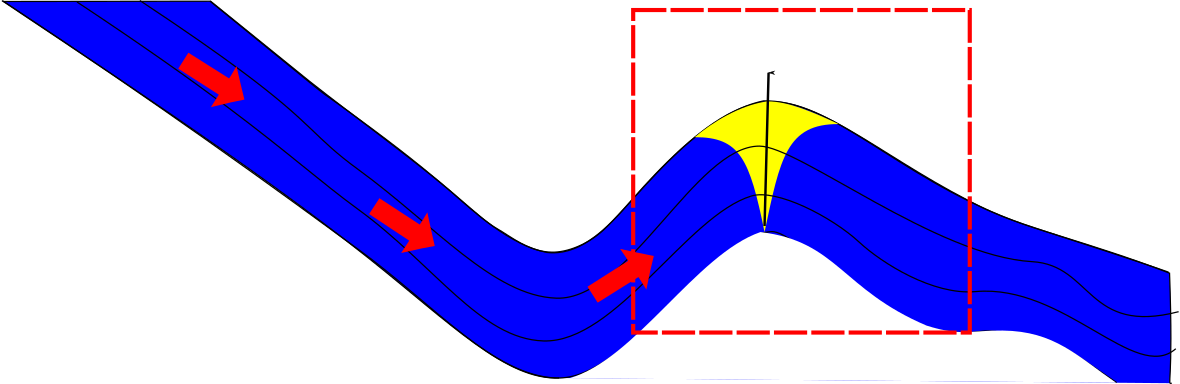
\includegraphics[width=0.65 \linewidth]{./figurer/bkw} 
  %
  \caption{External pressure drive.}
  \label{fig:bkw}
%
\end{figure}


\section{Flow modeling}

We use a standard porous media simulator to solve the flow equations in the medium. The solution is based on finite difference method and the following assumptions are taken:

\begin{itemize}

  \item Two compressible phases are considered in the medium: water and super critical ${CO}_2$.
  \item No mass exchange occurs between the two considered phases.
  \item No heat exchange is considered.

\end{itemize}

All of the realizations have dimensions of $3~\mbox{km}~\times~9~\mbox{km}~\times~80~\mbox{m}$, which is enough to capture variations in the designed geological features. While the scale of the used realizations is reasonably enough to capture the $\mbox{CO}_2$ distribution in the medium, the pressure disturbance imposed by the injector can go beyond this scale. To compensate for the size, we choose hydrostatics boundary conditions for the models. The open boundaries are modeled by considering a huge pore volume for the outer cells in the model that represent the boundary. Fig. shows the boundary condition defined in the model.

We consider $20\%$ of the total model pore volume for injection, which amounts to $40~\mbox{MM m}^3$. This volume is injected into realizations in three different scenarios. In the first scenario, the injection is forced in $30~\mbox{years}$ time scale and the pressure in the system is allowed to rise unlimitedly. Linear relative permeability functions are considered in this scenario. The purpose of first scenario is to examine the flow distribution in the medium influenced by geological heterogeneity. Linear assumption for relative permeabilities is taken to speed up the flow within the medium. The relative permeability curvature has shown a significant influence on the pressure behavior in the  aquifer. 

In the second scenario, the injector operates with the same fixed rate as in the first scenario and the relative permeability curve is chosen to be a quadratic function. A quadratic relative permeability curve causes lower flow mobility in the medium compared to the linear function, and by forcing the injector with a fixed volumetric rate of injection, the pressure rises significantly in the aquifer. This leads us to the third injection scenario, where the injector is controlled by pressure rather than volumetric rate. Thus, injection time is variable depending on the injectivity of the medium.

Only one injector is considered in the study. With one injector, it is easier to study the flow behavior and the plume development within the medium. It is located in the flank and in order to increase the sweep efficiency for the up-moving $\mbox{CO}_2$ plumes, the injector is completed in the lower part of the aquifer. The injector location and the completed layers are fixed for all of the realizations. The studies here aim to identify the influence of uncertainty on injectivity and fixing a place for injection helps in achieving this goal. In a deterministic case, we can complete the well in the best quality layers. 

There are few locations of distorted geometries in the faulted realizations that may be considered as structural traps for the injected $\mbox{CO}_2$. The topography in the SAIGUP realizations is simple and does not cover the variational space to be used in a sensitivity analysis. The slight inclination in the structural geometry of the medium, from the flank up to the crest, leads the injected $\mbox{CO}_2$  to accumulate in the crest and below the faulted side of the aquifer.

In a homogeneous medium, we expect the $\mbox{CO}_2$ to accumulate under the cap-rock. A small fraction of the injected $\mbox{CO}_2$ will escape through the open boundary near the injection well and the rest of it will stay within the medium in two forms that we refer to them as  mobile and residual volumes. As the $\mbox{CO}_2$ moves through the rock, part of it stays in the smaller pores by capillary trapping process and can not be discharged by brine. The the other parts move through the larger pores and can be displaced by water in an imbibition process. This volume is called mobile. As we are interested in storing the $\mbox{CO}_2$ permanently and safely, increasing the trapped volume is in lined with the objective of minimizing the leakage risk and maximizing the storage capacity. Likewise, the more mobile volume of $\mbox{CO}_2$ exists in the medium, the more will be the risk of leakage. 

\subsection{Flow responses}

The main flow equation unknowns considered here are the $\mbox{CO}_2$ pressure and the saturation distribution at different times. We extract quantities that address the feasibility of $\mbox{CO}_2$ injection from the simulation outputs. These quantities include a number of flow responses related to the $\mbox{CO}_2$ injection and migration problems. Each of these responses are directly or indirectly a measure for success of the operation within a specific realization. In the followings, we give a brief description of each of them.

\textbf{\textit{Boundary fluxes:}}

The flux out of open boundaries is a measure of sweep efficiency for the
CO$_2$ plume. Channeling can lead to early CO$_2$ breakthrough at boundaries and we prefer cases with less out-fluxes through open boundaries. The out-flux through the down open boundary, which is closer to the injector, is a potential loss for the injected volume. After the injector stops, some of the CO$_2$ that have left the domain comes in again due to gravity segregation effect. 

\textbf{\textit{Total mobile and residual $\mbox{CO}_2$ volume:}}
If the CO$_2$ saturation is below the critical value, it will be immobile in the
bulk flow, although not in the molecular sense. Less mobile CO$_2$ means less
risk of leakage and more residual volumes (with saturations less than the
critical) resulting from a more efficient volume sweep as preferable. We use critical saturation of 0.2 for both water and CO$_2$. During injection time the flow process is mainly drainage but after injection imbibition also happens and increases the residual trapped CO$_2$. 

\begin{figure}[thb]
  \centering
  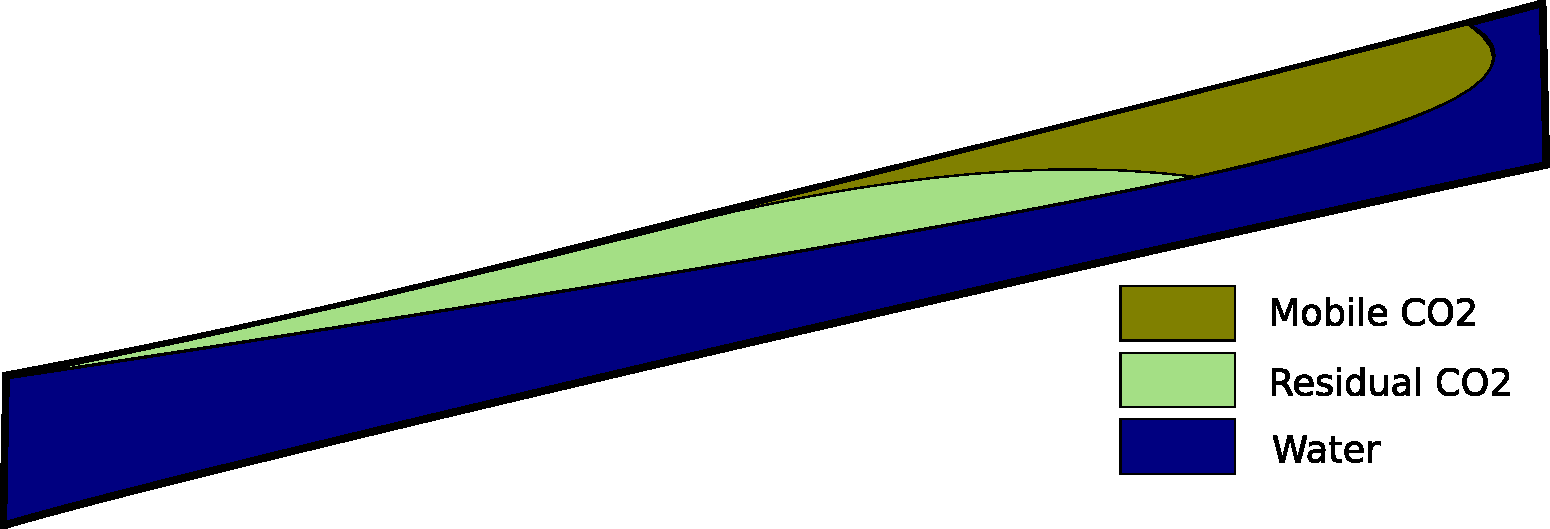
\includegraphics[width=0.65 \linewidth]{./figurer/MobRes} 
  %
  \caption{Mobile and residual CO$_2$ volume.}
  \label{fig:MobRes}
%
\end{figure}

\textbf{\textit{Total number of $\mbox{CO}_2$ plumes and largest plume:}}
To estimate the risk of leakage from the cap-rock, we assume that all mobile
CO$_2$ connected to a leakage point will escape out of the reservoir. Hence, it
is preferable if the total mobile CO$_2$ volume is split into smaller plumes
rather than forming a big mobile plume. Though the area exposed to potential
leakage points will increase by splitting the plume, yet the volume reduction is
overtaking the area effect. We looked at the largest plume size, the number of plumes, and other statistical parameters. 

% 
% \begin{figure}[thb]
%   \centering
%   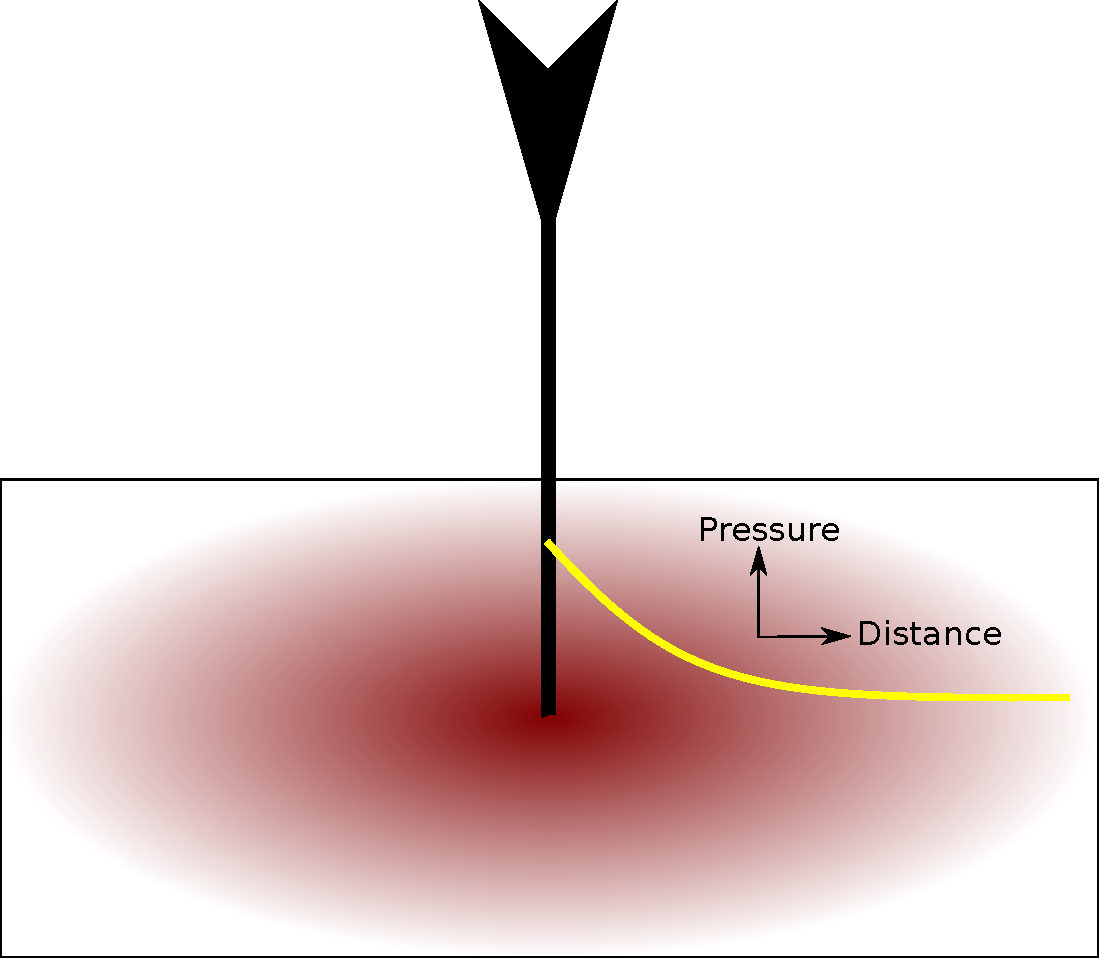
\includegraphics[width=0.65 \linewidth]{./figurer/NWB} 
%   %
%   \caption{NWB.}
%   \label{fig:nwb}
% %
% \end{figure}

\textbf{\textit{Average aquifer pressure:}} 

Average aquifer pressure is one of the most important responses to be considered. The pressure response in general shows a sharp jump at the start of injection and a declining trend during the injection and plume migration.  

As soon as the injection starts, a pulse of pressure goes through medium making a pressure buildup in the aquifer. When the pressure wave reaches the open boundary, the aquifer pressure starts declining to a level maintained by the injector. When the injector stops operation, the pressure support will be removed and the pressure drops and declines until it reaches equilibrium.

\textbf{\textit{Leakage risk:}}

During injection operation the foremost important issue is the aquifer pressure which as discussed earlier may lead to fractures in the cap-rock. On the other hand the cap-rock break depend on lithology and sealing thickness and differs from point to point. Some weaker locations can be the most probable to
break and start leaking if any mobile CO$_2$ exists there.

Geomechanical modeling of aquifer combined with flow modeling in the medium are far more costly to be implemented thoroughly in sensitivity, uncertainty and risk analysis. To avoid huge calculations, the idea is to model the possible breakings on the cap-rock (considering the stress stream in the medium) by introducing a probability measure on the cap-rock. This measure can be used to evaluate different cases for their risk of leakage, considering the CO$_2$ distribution under the cap-rock. 

Here we define the probability of leakage as a measure on the cap-rock that assigns a value to each point of cap-rock modeling the relative weakness of the cap-rock and the medium on that point. If for example both the cap-rock and the aquifer are continuous homogeneous layers with constant thickness, then the point of cap-rock which sits on the toppest point of the injection slice can be the most probable place for leakage in case of dramatic pressure increase in the well: the stress stream is more in the injection slice and the CO$_2$ accumulation occurs on the topmost part of the mentioned slice. Then one may consider a 2D-Gaussian probability distribution on the cap-rock, centered above the injection slice.

If the medium is heterogeneous or tilted, the injected CO$_2$ may be distributed in different number and sizes of plumes below the cap-rock. Therefor, in addition to the probability of breaking for each point of cap-rock, one must consider the CO$_2$ connected volume which is attached to that point. 

Since we have neither the cap-rock model nor the geomechanical properties of SAIGUP models, we use a simple 2D-Gaussian leakage probability distribution centered at a point on the crest which is in the same slice of injection point (Fig. \ref{fig:SLR}). We calculate the probability of each cell on the top layer and using the simulation results for the case, we weight it by the CO$_2$ saturation of that cell and the plume size which that cell is attached to. Summing up the values of the topmost cells, we assign a single number to the case which we call leakage risk of the case. One may weight the case risk value with the average pressure in the system, such that higher pressure gives a bigger weight.

One way to report the described responses and their relations to the uncertain parameters in one graph is to use scatter plots. Each case then will be represented by a marker sign with attributes dedicated to the set of geological parameter levels used in that case. Figure~\ref{fig:codes} shows some of the codes used in the study.


\begin{figure}
  \centering
  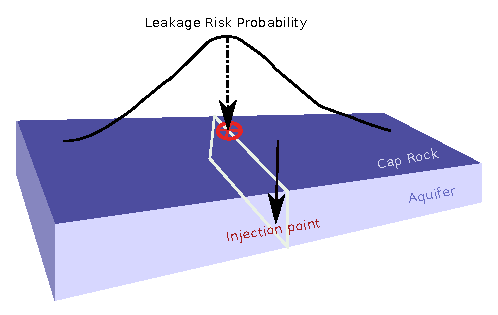
\includegraphics[width=0.65 \linewidth]{./figurer/LR_2} 
  %
  \caption{gauss.}
  \label{fig:SLR}
%
\end{figure}


\begin{figure}
  \centering
  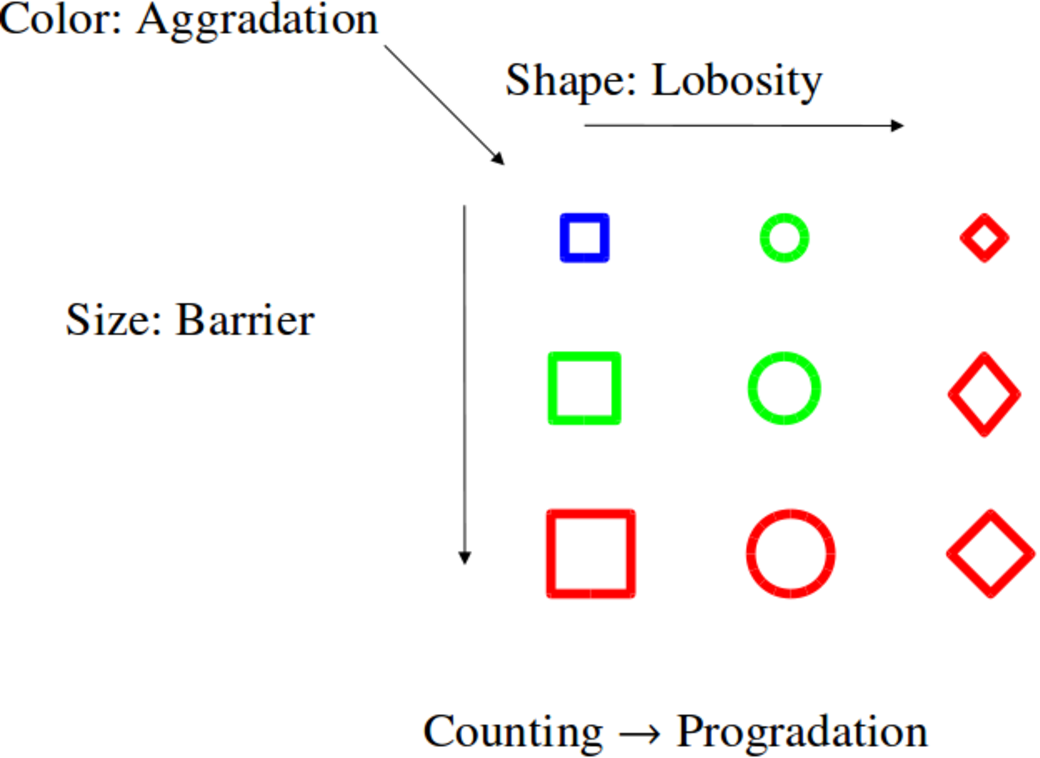
\includegraphics[width=0.65 \linewidth]{./figurer/codes} 
  %
  \caption{Marker codes used to plot the simulation results of all cases together.}
  \label{fig:codes}
%
\end{figure}


\section{Stochastic analysis}

In practice, modeling complicated physical phenomena is a stochastic process. Uncertainty can exist in different parts, from the model input parameters to the formulation of dependency rules in the model. Uncertainty coming from any source in the modeling propagates through the system response predictions. Ranking the important parameters in the modeling based on their influence in the responses can help in understanding the system and treating the stochastic nature of the process. Identifying and evaluating the uncertainties and their impact is a significant task and sensitivity analysis is known to be the right approach to identify the significance of uncertainty sources within modeling and to improve understanding of model behavior. The European Commission and the United States Environment Protection Agency recommend using sensitivity analysis in the context of extended compact assessment for policy making \cite{saltelli4global}.

Uncertainty sources within $\mbox{CO}_{2}$ storage problem can exist in different types as geological, physical and operational. This work is devoted to the geological uncertainties, however the same procedure can be applied to extend the work for other types. Here, we use a set of SAIGUP realizations to practice sensitivity analysis and how to assess the risk accompanied by uncertainties in the modeling. 

We use the stochastic response surface method to project solutions into space of high-dimensional polynomials via arbitrary polynomial chaos expansion \cite{oladyshkin2011concept}. The orthogonal polynomial bases can be constructed according to arbitrary probability space of the uncertain parameters. The reduced model represented by the response surface is vastly faster than the original complex one, and thus provides a promising starting point for global sensitivity analysis and probabilistic risk assessment.  

Some sensitivity analysis methods are robust only for linear problems and fail in extrapolating a nonlinear behavior. Some of them demonstrate local sensitivity and fail to cover the entire variation of input variable space. If some of the parameters with considerable influence are fixed in the study, the sensitivity study can be misleading. Increasing number of input variables gives more variation in output. However, this must be combined with a justification in selecting parameters based on available knowledge to increase the efficiency of the analysis. 

A practical approach in sensitivity analysis is to work with variances. This approach shows a good success in nonlinear problems \cite{reuter2008global}. When the system is decomposed into approximated functions, it is easy to implement methods based on variance. In our case, the variance in output responses can be set equal to variance of polynomial components calculated for each input parameter. In the current paper we use Sobol indices \cite{sobol2001global} for sensitivity analysis. The fact that the response surface has known polynomial properties \cite{OladNowakBarros_AWR2011} can further simplify these tasks. And finally, we perform risk analysis by using Monte-Carlo procedure. The approximating polynomial is fast enough to be used for large number of simulations. This makes it possible to have big range of variations in the output and easier interpretations of risk in the system. We conclude by a discussion on the results.
%==========================================================================



\subsection{Response surface via arbitrary polynomial chaos expansion}

Working with huge amounts of uncertainty puts demand for stochastic tools to analyze the system and the propagation of uncertainties through system output. Stochastic response surface is one such tool. Obviously, a response surface can be constructed in different ways, e.g. it can be constructed directly on a dense Cartesian grid of input parameters at extremely high computational efforts. Likewise, conceptually straightforward numerical Monte Carlo (MC) simulation techniques are computationally demanding since the statistical accuracy of their predictions depend on the number of realizations used. We explore an alternative methodology which demands only minimum number of model evaluations to construct a response surface. This approach is based on theory of polynomial chaos expansion (PCE) introduced by \cite{Wiener1938}. The basic idea is to represent the response of a model to changes in variables through a response surface that is defined with the help of an orthonormal polynomial basis in the parameter space.  In simple words, the dependence of model output on all relevant input parameters is approximated by a high-dimensional polynomial.  This projection can be interpreted as an advanced approach to statistical regression.  The PCE offers an efficient and accurate high-order way of including non-linear effects in stochastic analysis, see e.g. \cite{Zhang_Lu_2004_JCP,foo_pcm_JCP2010, Fajraoui_al_2011_WRR}. One of the attractive features of PCE is the high-order approximation of error propagation \cite{Ghanem_Spanos_1990_PC_in_SFEM,Ghanem_Spanos_1991_SFEM_book} as well as its computational speed when compared to MC \cite{oladyshkinintegrative}. 

To accommodate for a wide range of data distributions, a recent generalization of PCE is the arbitrary polynomial chaos (aPC), see e.g. \cite{oladyshkin2011concept}. Compared to earlier PCE techniques, the aPC adapts to arbitrary probability distribution shapes of input parameters and, in addition, can even work with unknown distribution shapes when only a few statistical moments can be inferred from limited data or from expert elicitation. They can be specified either analytically (as probability density/cumulative distribution functions), numerically as histogram or as a raw data sets. The aPC approach provides improved convergence in comparison to classical PCE techniques, when applied to input distributions that fall outside the range of classical PCE. 

Suppose that we approximate a problem by functional $\Upsilon$, which gives responses $\Gamma$ for input variables $\Theta$:
%
\begin{equation}
  \Gamma=\Upsilon(\Theta),
  \label{eq:1}
\end{equation} 
%
we define $h$ as a mapping from random variable space $\xi$ to random input space $\Theta$. This represents the uncertainty in the input data:
%
\begin{equation}
  \Theta=h(\xi).
  \label{eq:rand}
\end{equation}
%

Parametric mathematical expressions are used for approximation. In our case, we use a polynomial expansion which has some coefficients. These coefficients do not necessarily have a direct physical interpretation. Instead, we must tune the polynomial coefficients such that the prediction by our polynomial functional matches some available realistic responses. These responses, if not available from real measurements, are calculated in a physical law based modeling for a set of input data. Hereby, we rewrite the functional (\ref{eq:1}) to show its dependency on data driven parameters:
%
\begin{equation}
  \Gamma=\Upsilon(\Theta)=\upsilon(\Theta,\alpha).
  \label{eq:parm}
\end{equation}
%
Here, $\Theta$ is in the input variable space and $\alpha$ is in the data driven parameter space, that represents the dependency between input and output of the system\footnote{An example of data driven parameter space is the polynomial coefficient space in approximating by polynomials.}. First we specify $\alpha$. Then given $\Theta$, the responses $\Gamma$ can be estimated. In many practical problems, input parameters are expressed in terms of random variables and a functional form is defined to quantify the system responses. This functional expression can be in different forms, from simple linear mapping to very complicated non-linear forms. 

Considering the uncertainty of input, the aPC constructs a set of polynomial base functions and expand the solution into a space of these bases. Thus, the response vector $\Gamma$ in Eq.~(\ref{eq:1}) can be approximated by: 
%
\begin{equation}
\Gamma\approx\underset{i=1}{\overset{n}{\sum}}c_{i}\underset{t=1}{\overset{n_c}{\prod}}P_{i,t}(\theta_{t}).
  \label{eq:exp}
\end{equation} Here, $n$ is the considered number of modeling parameters, $n_c$ is the number of expansion terms, $c_{i}$ are the expansion coefficients, and $P_{i,t}$ are the multi-dimensional polynomials of order $t$ for the variables $\theta_{t}$, $\Theta=[\theta_{1},...,\theta_{n}]$. The polynomials $P_{i,t}$ are defined as : 
\begin{equation}
P_{i,t}=\underset{}{\overset{}{\underset{q=0}{\overset{i}{\sum}}}p_{q,t}\theta^{q}_t}. \label{eq:bases}\end{equation}
%
The number $n_c$ of unknown coefficients $c_{i}$ depends on the degree d of the approximating polynomial, and the number of considered parameters $n$:
%
\begin{equation}
 n_c=\frac{(d+n)!}{d!\times n!}.
 \label{eq:np}
\end{equation}
%
%---------------------------

%##################################


\subsubsection{Data-driven orthonormal basis}

All orthogonal polynomials in the expansion (\ref{eq:exp}) fulfill the following condition:
%
\begin{equation}
\int_{I\in\Omega}\omega P_{l}P_{m}d\tau(\Theta)=\delta_{lm},\label{eq:orth}\end{equation} where $\omega$ is a weight function, $\delta$ is the Dirac function, and $\tau$ is the measure for input variable space. We choose the weight to be one, i.e., $\omega\equiv1$. 

According to \cite{oladyshkin2011concept} the orthogonal polynomial basis satisfying Eq.~(\ref{eq:orth}) can be obtained from the solution of the following linear system of equations: 
%
\begin{equation}
\left[\begin{array}{cccc}
\mu_{0} & \mu_{1} & ... & \mu_{k}\\
\mu_{1} & \mu_{2} & ... & \mu_{k+1}\\
... & ... & ... & ...\\
\mu_{k-1} & \mu_{k} & ... & \mu_{2k-1}\\
0 & 0 & ... & 1\end{array}\right]\left[\begin{array}{c}
P_{0}^{(k)}\\
P_{1}^{(k)}\\
...\\
P_{k-1}^{(k)}\\
P_{k}^{(k)}\end{array}\right]=\left[\begin{array}{c}
0\\
0\\
...\\
0\\
1\end{array}\right],\label{eq:orthsys}\end{equation} in which $P_{q}^{(k)}$ corresponds to $p_{q,t}$ term in Eq.~\ref{eq:bases}, when it is written for $P_{k,t}$.
Here, $\mu_{k}$ is the $k^{th}$ non-central (raw) statistical moment of random input variable, which is defined as:
%
\begin{equation} \mu_{k}=\int_{\Theta\in\Omega}\Theta^{k}d\tau(\Theta).\label{eq:mnt}\end{equation}
%
Thus, arbitrary polynomial chaos expansion base on Eq.~\ref{eq:orthsys} only demands the existence of a finite number of moments, and does not require the exact knowledge or even existence of probability density functions. An interesting aspect is that only moments up to twice the order of expansion matter. This means, that there is no need for any kind of assumptions for data probability distribution leading to subjectivity artifacts as discussed earlier.

Uncertainty knowledge never is perfect such that we can express the probability of data values in a unique distribution function. Available data are mostly scarce and fitting a function to observed frequencies is biased. Oladyshkin et al. \cite{oladyshkin2011concept} used available data with no formal knowledge requirements for uncertainty distribution. Direct data values are not even used in the method. Instead, arbitrary orthogonal polynomial bases are constructed from statistical moments of the available data. This way, it is possible to calculate mean, variance, and higher order moments even with sparse data. 


\subsubsection{Non-intrusive determination of the coefficients}

Generally, all PCE techniques can mainly be sub-divided into
intrusive \cite{Ghanem1993,Matthies2005,Xiu2003} and non-intrusive \cite{Keese2003,Isukapalli1998,nLi2007,oladyshkinintegrative}
approaches, i.e., methods that require or do not require modifications in the system of governing equations and corresponding changes in
simulation codes. Intrusive approaches require symbolic manipulations of the governing
equations and can sometimes provide semi-analytical solutions for stochastic
analyses of simple problems. The most well-known method from this group is the
stochastic Galerkin technique. However, the necessary symbolic manipulations may
become very complex and analytically cumbersome, and cannot easily be
implemented in commercial codes. For this reason, non-intrusive approaches like
sparse quadrature and the probabilistic collocation method (PCM: see \cite{nLi2007,oladyshkinintegrative}) have lately been
receiving a quickly increasing attention. In a simple sense, PCM can be interpreted
as a smart (mathematically optimal) interpolation rule of model output between
different parameter sets. The polynomial interpolation may be interpreted as a
response surface of the model. It is based on a minimal and optimally chosen set of
model evaluations, each with a defined set of model parameters (called collocation
points). The challenge here is to find a compromise between computational effort and a
reasonable approximation of the physical processes.


The collocation formulation does not require any knowledge of the initial model structure. It only requires knowledge on how to obtain the model output for a given set of input parameters, which allows to treat the model  like a \textquotedblleft black-box\textquotedblright.  The distinctive feature of non-intrusive approaches is that any simulation model can be considered a ``black-box'', i.e. commercial software can be used without any modifications required.  According to \cite{Villadsen1978}, the optimal choice of collocation points corresponds to the roots of the polynomial of one degree higher ($d+1$) than the order used in the chaos expansion ($d$). This strategy is based on the theory of Gaussian integration (e.g., \cite{Abramowitz1965}). For one-dimensional integrations, it allows exact numerical integrations of order $d$ given $d+1$ values of the function to be integrated. 

For multi-parameter analysis, the number of available points from the original optimal integration rule is $(d+1)^n$, which is larger than the necessary number $M$ of collocation points. The full tensor grid can be used for low-order ($1^{st}$, $2^{nd}$) analysis of few parameters, but for higher-order analysis of many parameters the tensor grid suffers from the curse of dimensionality ($(d+1)^n$ points). In that case, a smart choice of a sparse subset of the tensor grid becomes necessary. For this reason, the collocation approach became more popular in the last years. Probabilistic collocation \cite{nLi2007, oladyshkinintegrative,oladyshkin2011concept} chooses the collocation points  from the full tensor grid according to their probability weight, i.e. their importance as specified by the available probability distribution of $\boldsymbol{\Theta}$. This simply means to select the collocation points from the most probable regions of the input parameters' distribution (see \cite{oladyshkinintegrative}) and the modeler can extract a lot of information in the main range of the parameter distribution (Figure~\ref{fig:col}).

\begin{figure}
  \centering
  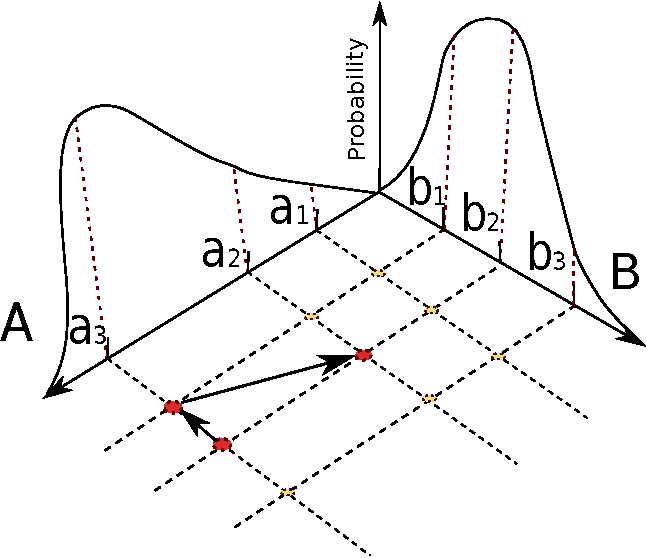
\includegraphics[width=0.65 \linewidth]{./figurer/col} 
  %
  \caption{Collocation points are combined in different uncertainty directions such that the total probability in all directions is maximized.}
  \label{fig:col}
%
\end{figure}

In our study we apply the probabilistic collocation method for computing the coefficients $c_{i}$ in Eq.~\ref{eq:exp}, which requires the minimum number of model evaluations. The weighted-residual method in the random space is defined as \cite{nLi2007}:

\begin{equation}
\int(\Gamma-\underset{i=1}{\overset{n_c}{\sum}c_{i}}\underset{t=1}{\overset{n}{\prod}}P_{i,t}(\theta_{t}))w(\Theta)p(\Theta)d\tau=0,\label{eq:residual}\end{equation}
where $w(\Theta)$ is the weighting function and $p(\Theta)$ is the joint probability density function of $\Theta$. In the probabilistic collocation method, the weighting function is chosen as the delta function:
\begin{equation}
 w(\Theta) = \delta(\Theta-\Theta_c). \label{eq:weight}
\end{equation}
$\Theta_c$ is the set of collocation points. Substituting from Eq.~\ref{eq:weight} into Eq.~\ref{eq:residual} gives the following:

\begin{equation}
 \Gamma_{c}-\underset{i=1}{\overset{n_c}{\sum}c_{i}}\underset{t=1}{\overset{n}{\prod}}P_{i,t}(\theta_{t,c})=0, \label{eq:solution}
\end{equation}
 where $\Gamma_c$ are the response values corresponding to the collocation values $\theta_{t,c}$, as the component $t$ of $\Theta_{c}$. We solve Eq.~\ref{eq:solution} to find coefficients $c_i$.

\subsection{Sensitivity analysis}
\label{Section:SA}
Sensitivity analysis helps in understanding the general role of parameters in models and the impact of varying model parameters on the response of prediction models. This understanding can be useful both in optimizing the system performance and in studying the variation in performance coming from the stochastic nature of the system. Global sensitivity analysis presents a trend of system behavior without being trapped in a local infimum. Some methods like the gradient based methods can lead to local minimum or maximum \cite{saltelli2007global}. Some sensitivity analysis methods work better with linear problems and some of them fail with nonlinearity. Variance based methods provide global sensitivity and work for general non-linear problems. When the response is decomposed into simpler components (for instance, in polynomial bases), the output variance can be corresponded to components. Component dependence to distinct variables specifies the contributions of input variables into the output variance. It is possible then to rank the input variables based on their contribution to the variance \cite{saltelli2007global,reuter2008global}.

In this Section, we tackle global sensitivity analysis based on the aPC technique, following the line of work on aPC by \cite{oladyshkin2011concept, OladNowakBarros_AWR2011}. Up to present, the Morris method \cite{Morris1991} considers a uniform importance of input parameters within pre-defined intervals. in current study we tackle a weighted global sensitivity, because the presented framework accounts for arbitrary bounds or weighting functions for input parameters.  The big advantage of aPC-based sensitivity analysis, is that one can obtain global sensitivity information at computational costs that are hardly larger than those for local analysis. The reason is the following: local methods use infinitesimally small spacing between parameter sets for model evaluation to get numerical derivatives evaluated at a single point. The aPC based-method places the parameter sets for model evaluation at an optimized spacing in parameter space. This can be interpreted as fitting secants (or polynomials for non-linear analysis) to the model response. These secants (polynomials) approximate the model over the entire parameter space in a weighted least-square sense (compare with the best unbiased ensemble linearizion approach described by \cite{Nowak_2009_BUEL}). This is more beneficial to computing a tangent or local second derivatives (compare FORM, SORM methods, e.g., \cite{Jang1994}) that approximate the model well just around one point in the parameter space.

In the following, we describe the Sobol sensitivity indices technique for quantification of relative importance of each individual input parameter in the final prediction. Then we implement the method for our geological $\mbox{CO}_{2}$ storage problem.
%---------------------------


\subsubsection{Sobol sensitivity indices}

As an advantage, in variance based methods one can work with arbitrary system as a black box and calculations are based on inputs and outputs only. However, economy of calculation is a challenge. The method is well described in the literature \cite{sobol2001global,saltelli2007global,saltelli4global,reuter2008global}. More recent works are concerned about expediting calculation pace \cite{crestaux2009polynomial,oladyshkin2011concept, OladNowakBarros_AWR2011}. The idea is to replace the system with an approximating function which gives benefits in sensitivity calculations.

Using polynomials in approximating solutions makes it convenient to perform sensitivity analysis, because it is easy to correspond the output variances to the input variables. The solution is approximated by orthogonal polynomial bases with increasing dimensionality. We expand the variance of output solution into components. Assume that we break the system output into components:

\begin{equation}
\Gamma=\Gamma_{0}+\underset{_{i}}{\sum}\Gamma_{i}+\underset{_{i}}{\sum}\underset{_{j>i}}{\sum}\Gamma_{ij}+...\label{eq:comp}\end{equation}

A single index shows dependency to a specific input variable. Wheres more than one index shows interaction of input variables. If we consider input vector $\Theta$ to be of $N$ components $\theta_{i}$ for $i=1,..,n$, then $\Gamma_{i}=f_{i}(\theta_{i})$ and $\Gamma_{ij}=f_{ij}(\theta_{i}\theta_{j})$. In practice, we stop at finite number of terms in Eq.~(\ref{eq:comp}).
 The first order sensitivity index, so called Sobol index, is defined as follows \cite{saltelli2007global}:

\begin{equation}
S_{i}=\frac{\mbox{V}[\mbox{E}(\Gamma\mid\theta_{i})]}{\mbox{V}(\Gamma)},\label{eq:sob1}\end{equation} where $\mbox{E}(\Gamma\mid\theta_{i})$ is the conditional expectation of output $\Gamma$ given $\theta_{i}$ and $\mbox{V}$ is the variance operator. Since $\theta_{i}$ can be fixed at any value in its uncertainty interval, each of those values produce a distinct expectation. In Eq.~(\ref{eq:sob1}), variance of those expectations is divided by variance of output with no fixed input variable. For more than one index, a higher-order Sobol index can be defined as:\begin{equation} S_{ij}=\frac{\mbox{V}[\mbox{E}(\Gamma\mid\theta_{i},\theta_{j})]-\mbox{V}[\mbox{E}(\Gamma\mid\theta_{i})]-\mbox{V}[\mbox{E}(\Gamma\mid\theta_{j})]}{\mbox{V}(\Gamma)}.\label{eq:sob2}\end{equation} Here, $\mbox{V}[\mbox{E}(\Gamma\mid\theta_{i},\theta_{j})]$ is the variance of output expectations after fixing $\theta_{i}$ and $\theta_{j}$. This index represents significance of variation in output generated from uncertainty in input variables together, i.e., the interaction of uncertain parameters. If we add all indices that contain variable $\theta_{i}$, the sum is called the total Sobol index:

\begin{equation}
S_{Ti}=S_{i}+\underset{_{j\neq i}}{\sum}S_{ij}+\underset{_{j\neq i}}{\sum}\underset{_{k\neq i}}{\sum}S_{ijk}+...\label{eq:totSob}\end{equation}


The total Sobol index can be used as a sensitivity measure to rank parameters for their influence in the results variation. When this index is close to zero, the corresponding parameter has negligible role in the variation of the system response. Therefore, the uncertainty in that parameter does not introduce a considerable error in the calculation of system responses. 

With known polynomial coefficients, Sobol indices are easy to calculate. When number of parameters is large, we do initial sensitivity analysis with lower degree polynomials to filter out pertinent parameters. Then the analysis continues on the filtered parameters with a higher
degree polynomial approximation.
%---------------------------

\subsection{Risk analysis}
\label{Section:RA}
Risk $R$ of a process is quantitatively defined as the extent of consequence $C$ caused by the process multiplied by the probability $P$ of that damage to happen:
%
\begin{equation}
R=P\times C\label{eq:rsk}.\end{equation}
%
The consequence can be defined by direct measures in the simulation responses, or it can be related to consequences of different flow scenarios. For example in the case of $\mbox{CO}_{2}$ injection into deep aquifers, the amount of $\mbox{CO}_{2}$ which stays mobile and undissolved in the medium for a time after injection can be considered as a consequence, bearing the potential of leakage up to the surface if exposed to a geological leakage point. The consequence could also be defined by a criterion for $\mbox{CO}_{2}$ injection scenario consequences, like the rate of climate change (either locally or globally) due to possible leakage of the stored $\mbox{CO}_{2}$, as the costs of pumping $\mbox{CO}_{2}$ that does not remain in the subsurface, or via the related costs for $\mbox{CO}_{2}$ emission certificates.

The other part is the probability of these consequences to happen. This depends on the stochastic behavior of the process which results in random outcomes. A conventional Monte-Carlo approach studies propagation of uncertainty through the system performance. Deterministic modeling is performed over a set of input data within the interval of uncertainty, drawn randomly from the respective probability distributions. 

Highly accurate MC analysis can be very costly in terms of computational expenses. We use the polynomial based reduced model, because it is fast enough to be used in a Monte-Carlo process. Thus, we can easily perform MC analysis with 10000 runs in a typical geological $\mbox{CO}_{2}$ storage problem. Thanks to the higher-order approximation via the aPC, the principal non-linear physical behavior of  $\mbox{CO}_{2}$ storage is included into analysis, and detailed probabilistic risk assessment becomes feasible.
%---------------------------

\begin{figure}[thb]
  \centering
  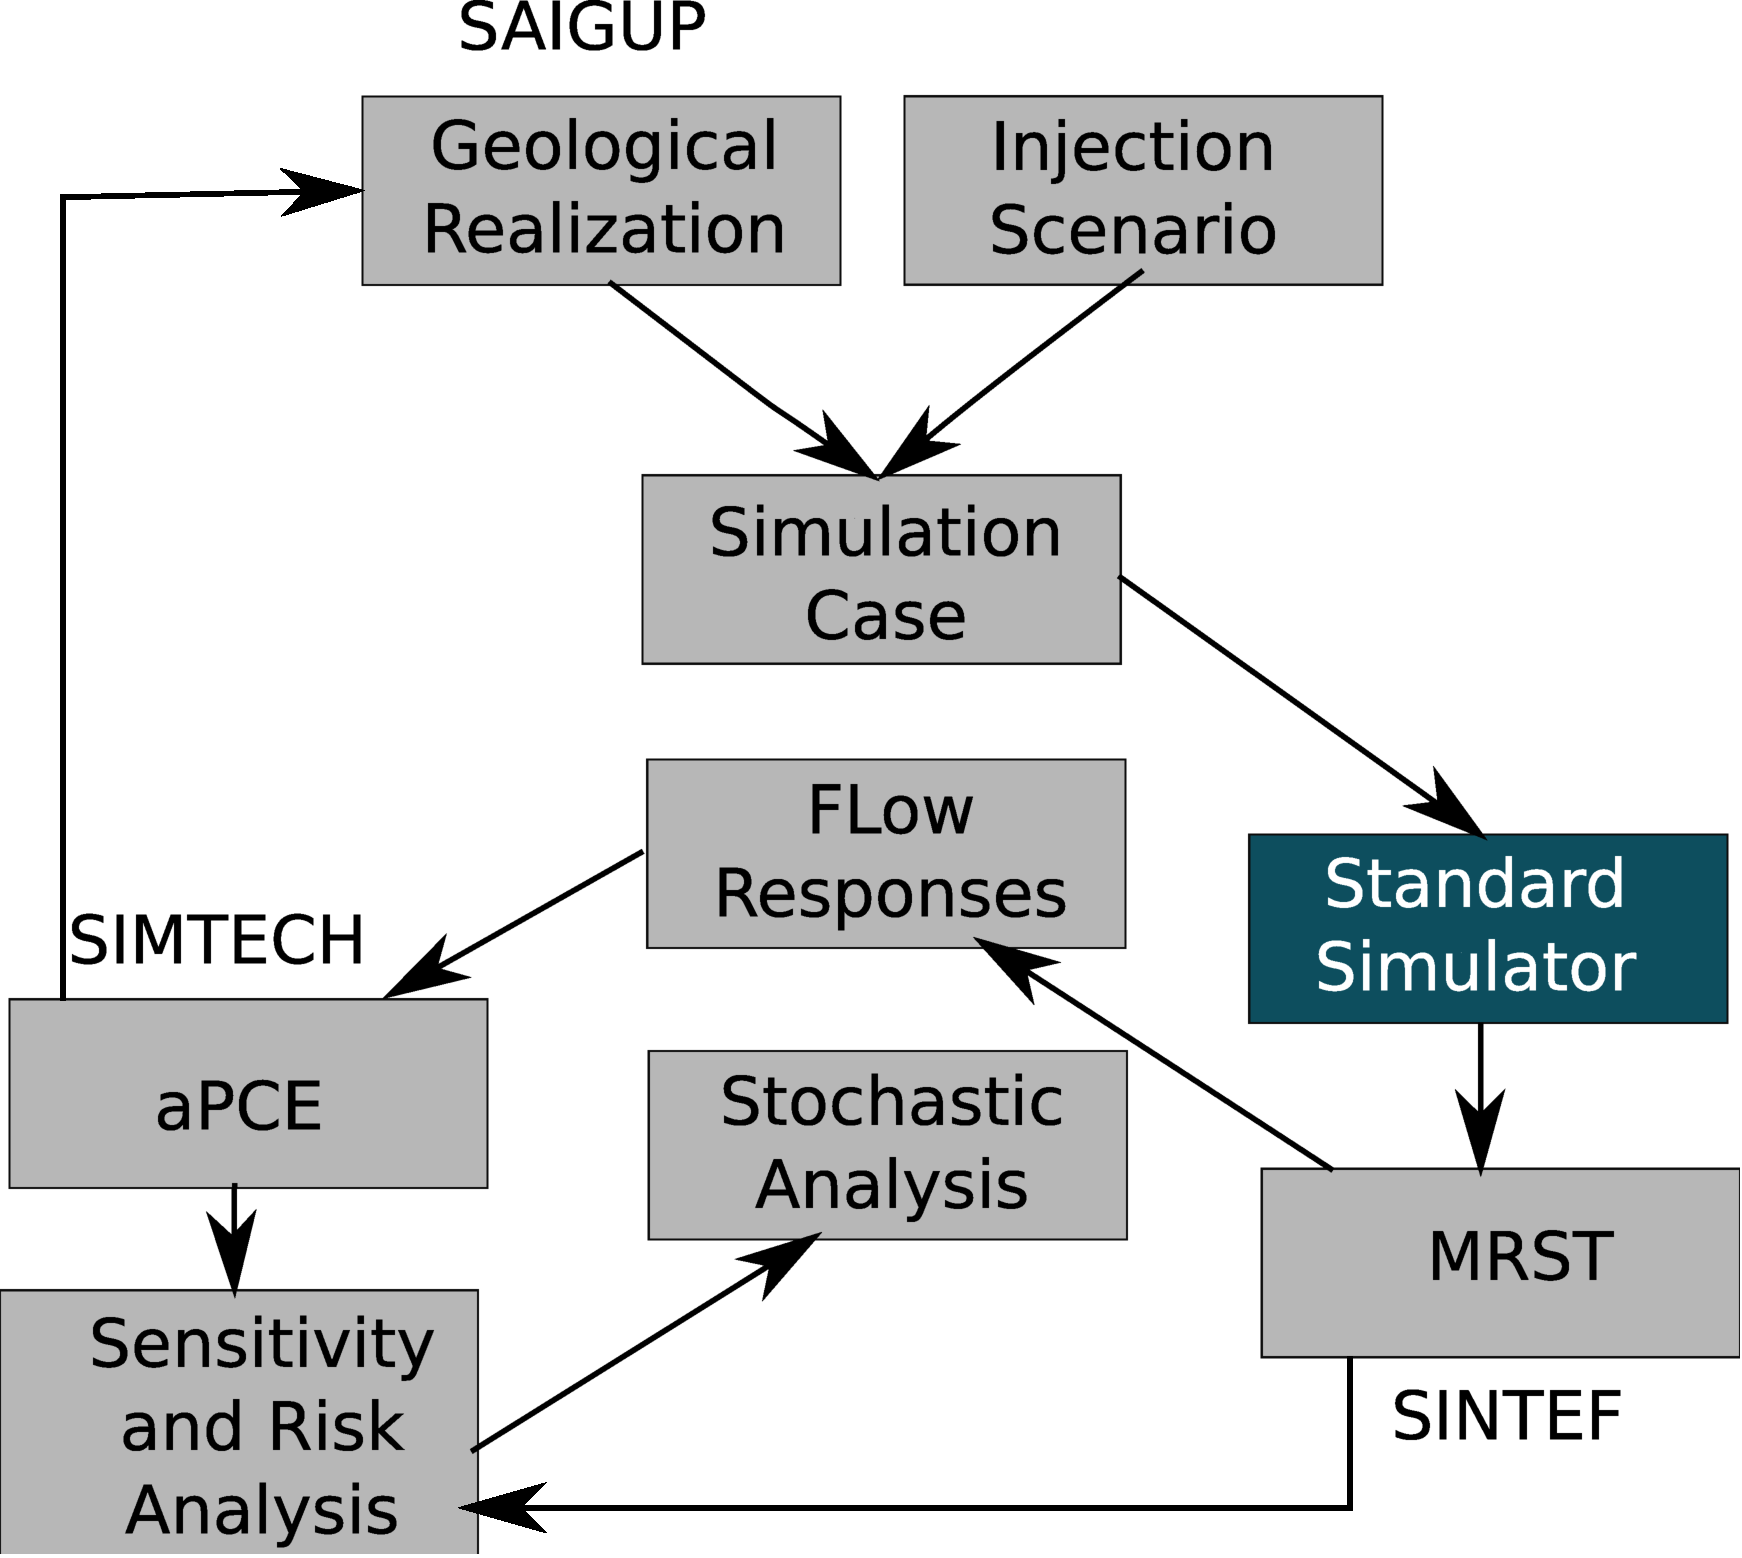
\includegraphics[width=0.65 \linewidth]{./figurer/ENCL} 
  %
  \caption{Flow-chart of work process implemented in an automated procedure.}
  \label{fig:encl}
%
\end{figure}

\section{Implementation work-flow}

This thesis incorporated working with large number of realizations, various flow scenarios, and different procedures and softwares. While the study progresses, new ideas and challenges rises that require manipulation of parts of the work-flow. In order to achieve the defined goals of the research, an automated work-flow is required that connects different parts of the study and converts data type in-between them. This makes the study feasible in terms of saving time for any necessary modifications.

Matlab programming language is used for implementing the work-flow in this research. The main reason for this choice, apart from the rich facilities available within Matlab toolboxes, is to use many axillary functions within Matlab Reservoir Simulation Toolbox (MRST) available as free software in Matlab language at SINTEF. For flow simulation a commercial software is used, which is a standard simulator for oil and gas industry and research. The simulator is using finite difference for flow modeling. Since the majority of numerical flow calculations are performed in this software, which is originally written in Fortran programming language, using Matlab for the study does not slow-down the simulation speed. 

Figure \ref{fig:encl} shows the elements of the work-flow implemented by a large number of Matlab functions. Functions from MRST at SINTEF and the stochastic tools of SIMTECH group in Stuttgart university are utilized and merged into the work-flow. The design is made such that the work-flow is flexible and general. Some research has been done by replacing the commercial simulator with in-house simulators at SINTEF, but the main study was performed using the black-box commercial simulator. 
